\documentclass[xcolor=dvipsnames,aspectratio=169]{beamer}
\usepackage[utf8]{inputenc}
\usetheme{Warsaw}
\usepackage{pgfpages}

% -----------------------------------------------------------------------------
% Notes toggle
% Compile with \def\NOTES{} before \input if you want notes-only output.
% -----------------------------------------------------------------------------
\newif\ifnotes
\ifdefined\NOTES\notestrue\fi
\ifnotes
  \setbeameroption{show only notes}
\else
  \setbeameroption{hide notes}
\fi

% -----------------------------------------------------------------------------
% Shared formatting
% -----------------------------------------------------------------------------
\setcounter{tocdepth}{2}

% =============================================================================
% Theme settings
% =============================================================================

% --- Core theme colors ---
\definecolor{ThemePrimary}{rgb}{0.0745, 0.1608, 0.2941}   % deep blue
\definecolor{ThemeSecondary}{rgb}{0.8667, 0.2039, 0.0118} % warm red/orange
\definecolor{ThemeAccent}{rgb}{0.1137, 0.3451, 0.6549}    % medium blue
\definecolor{ThemeLight}{rgb}{0.9725, 0.9804, 0.9882}     % near white
\definecolor{ThemeText}{rgb}{0.10, 0.10, 0.10}

% --- Optional extra palette ---
\definecolor{ThemeHighlight}{rgb}{0.9608, 0.5294, 0.1176}
\definecolor{ThemeSoftBlue}{rgb}{0.0000, 0.6235, 0.8314}
\definecolor{ThemeSoftNavy}{rgb}{0.1176, 0.2196, 0.4667}

% =============================================================================
% Beamer color settings
% =============================================================================

\setbeamercolor{palette primary}{bg=ThemePrimary,fg=ThemeLight}
\setbeamercolor{structure}{fg=ThemePrimary}
\setbeamercolor{section in toc}{fg=ThemePrimary}
\setbeamercolor{frametitle}{bg=ThemeSecondary,fg=ThemeLight}
\setbeamercolor{frametitle right}{bg=ThemePrimary}
\setbeamercolor{titlelike}{bg=ThemeSecondary,fg=ThemeLight}

% Optional tweaks you can enable later if desired:
% \setbeamercolor{block title}{bg=ThemePrimary,fg=ThemeLight}
% \setbeamercolor{block body}{bg=ThemeLight,fg=ThemeText}
% \setbeamercolor{section in head/foot}{bg=ThemeSoftNavy,fg=ThemeLight}
% \setbeamercolor{subsection in head/foot}{bg=ThemePrimary,fg=ThemeLight}

% =============================================================================
% Footline with page numbers
% =============================================================================

\defbeamertemplate*{footline}{shadow theme}{
    \leavevmode
    \hbox{%
        \begin{beamercolorbox}[
            wd=.5\paperwidth,
            ht=2.5ex,
            dp=1.125ex,
            leftskip=.3cm plus1fil,
            rightskip=.3cm
        ]{author in head/foot}
            \usebeamerfont{author in head/foot}\hfill\insertshortauthor
        \end{beamercolorbox}%
        \hskip0pt%
        \begin{beamercolorbox}[
            wd=.5\paperwidth,
            ht=2.5ex,
            dp=1.125ex,
            leftskip=.3cm,
            rightskip=.3cm plus1fil
        ]{title in head/foot}
            \usebeamerfont{title in head/foot}%
            \insertshorttitle\hfill\insertframenumber\,/\,\inserttotalframenumber
        \end{beamercolorbox}%
    }
    \vskip0pt
}

% =============================================================================
% Headline with current section / subsection
% =============================================================================

\setbeamertemplate{headline}{%
  \leavevmode
  \hbox{%
    \begin{beamercolorbox}[
        wd=.5\paperwidth,
        ht=2.1ex,
        dp=0.7ex,
        leftskip=0.3cm
    ]{section in head/foot}
      \usebeamerfont{section in head/foot}\insertsectionhead
    \end{beamercolorbox}%
    \begin{beamercolorbox}[
        wd=.5\paperwidth,
        ht=2.1ex,
        dp=0.7ex,
        rightskip=0.3cm
    ]{subsection in head/foot}
      \usebeamerfont{subsection in head/foot}\hfill\insertsubsectionhead
    \end{beamercolorbox}%
  }%
}

% =============================================================================
% Automatic outline slides
% =============================================================================

\AtBeginSection[]{
    \begin{frame}{Outline}
        \tableofcontents[currentsection]
    \end{frame}
}

\AtBeginSubsection[]{
    \begin{frame}{Outline}
        \tableofcontents[currentsection,currentsubsection]
    \end{frame}
}

% =============================================================================
% Figure / table packages
% =============================================================================

\usepackage{graphicx}   % figures
\usepackage{float}      % figure/table placement
\usepackage{rotating}   % rotated figures/tables
\usepackage{caption}    % captions
\usepackage{subcaption} % subfigures
\usepackage{makecell}   % table formatting
\usepackage{longtable}  % multipage tables
\usepackage{array}      % custom columns
\usepackage{tabularx}   % flexible-width tables
\usepackage{booktabs}   % professional tables

\newcolumntype{L}{>{\raggedright\arraybackslash}m{4cm}}
\newcolumntype{R}[1]{>{\raggedright\arraybackslash\hspace{0pt}\vspace{-0.25cm}}p{#1}}

% =============================================================================
% Math packages
% =============================================================================

\usepackage{amsfonts}
\usepackage{mathrsfs}
\usepackage{amsmath}
\usepackage{amssymb}
\usepackage{amsthm}
\usepackage{mathtools}
\usepackage{steinmetz}

% =============================================================================
% Chemistry / units
% =============================================================================

\usepackage[version=4]{mhchem}
\usepackage{chemformula}

\usepackage{siunitx}
\sisetup{locale = DE}
\sisetup{output-decimal-marker = {.}}

% =============================================================================
% Code / URL / verbatim
% =============================================================================

\usepackage{listings}
\usepackage{url}
\usepackage{verbatim}

% =============================================================================
% Badges (tractable / intractable / approximate)
% =============================================================================

\usepackage{pifont}

\newcommand{\badgeT}{\begingroup\setlength{\fboxsep}{1pt}\colorbox{ForestGreen!15}{\footnotesize\textcolor{ForestGreen}{\ding{51}\,Tractable}}\endgroup}
\newcommand{\badgeI}{\begingroup\setlength{\fboxsep}{1pt}\colorbox{BrickRed!15}{\footnotesize\textcolor{BrickRed}{\ding{55}\,Intractable}}\endgroup}
\newcommand{\badgeA}{\begingroup\setlength{\fboxsep}{1pt}\colorbox{BurntOrange!15}{\footnotesize\textcolor{BurntOrange}{\ding{72}\,Approx./Learned}}\endgroup}

% tiny inline versions (use in dense math)
\newcommand{\tbadgeT}{\textcolor{ForestGreen}{\scriptsize\ding{51}}}
\newcommand{\tbadgeI}{\textcolor{BrickRed}{\scriptsize\ding{55}}}
\newcommand{\tbadgeA}{\textcolor{BurntOrange}{\scriptsize\ding{72}}}

% =============================================================================
% End of format file
% =============================================================================


% -----------------------------------------------------------------------------
% Presentation metadata
% Update these for each new talk.
% -----------------------------------------------------------------------------
\newcommand{\TalkTitle}{Generative Models}
\newcommand{\TalkAuthor}{Soo Min Kimm}
\newcommand{\TalkInstitute}{}
\newcommand{\TalkDate}{07/11/25}

\title{\TalkTitle}
\author{\TalkAuthor}
\institute{\TalkInstitute}
\date{\TalkDate}

\begin{document}
    \begin{frame}
        \titlepage
		
		\note{Welcome everyone. Today I'll be presenting on generative models, which are a fundamental class of machine learning models that learn to model and generate data distributions. 
			  This topic is crucial in modern AI as generative models power many applications including image generation, text synthesis, and data augmentation. 
			  We'll explore various families of generative models, understanding their mathematical foundations, architectures, and trade-offs between different approaches. 
			  Each model family has its own strengths and weaknesses, making them suitable for different applications. 
			  We'll cover explicit models like autoregressive models and VAEs, implicit models like GANs, and score-based models like diffusion. 
			  The mathematical foundations we'll explore include variational inference, maximum likelihood estimation, and adversarial training. 
			  Let's begin our journey through the fascinating world of generative models.}
    \end{frame}
    
    \begin{frame}{Outline}
        \tableofcontents
		
		\note{The presentation is organised into three main sections. First, I'll cover the motivation for generative models, discussing the fundamental problem we're trying to solve and the constraints we face. 
			  We'll explore why generative modeling is important and what makes it challenging from a computational perspective. 
			  Then, I'll dive into different model families, including autoregressive models, VAEs, normalizing flows, flow matching, energy-based models, diffusion models, score-based models, and GANs. 
			  Each model family addresses the fundamental challenge of modeling probability distributions in different ways. 
			  We'll see how some models use explicit likelihoods while others use implicit distributions. 
			  Some models work with tractable computations while others approximate intractable integrals. 
			  Finally, I'll provide a comprehensive summary comparing these approaches in terms of their architectures, strengths, and limitations.}
    \end{frame}
    
    \section{Motivation}
        \begin{frame}{Intuition}
            \begin{figure}
                \centering
                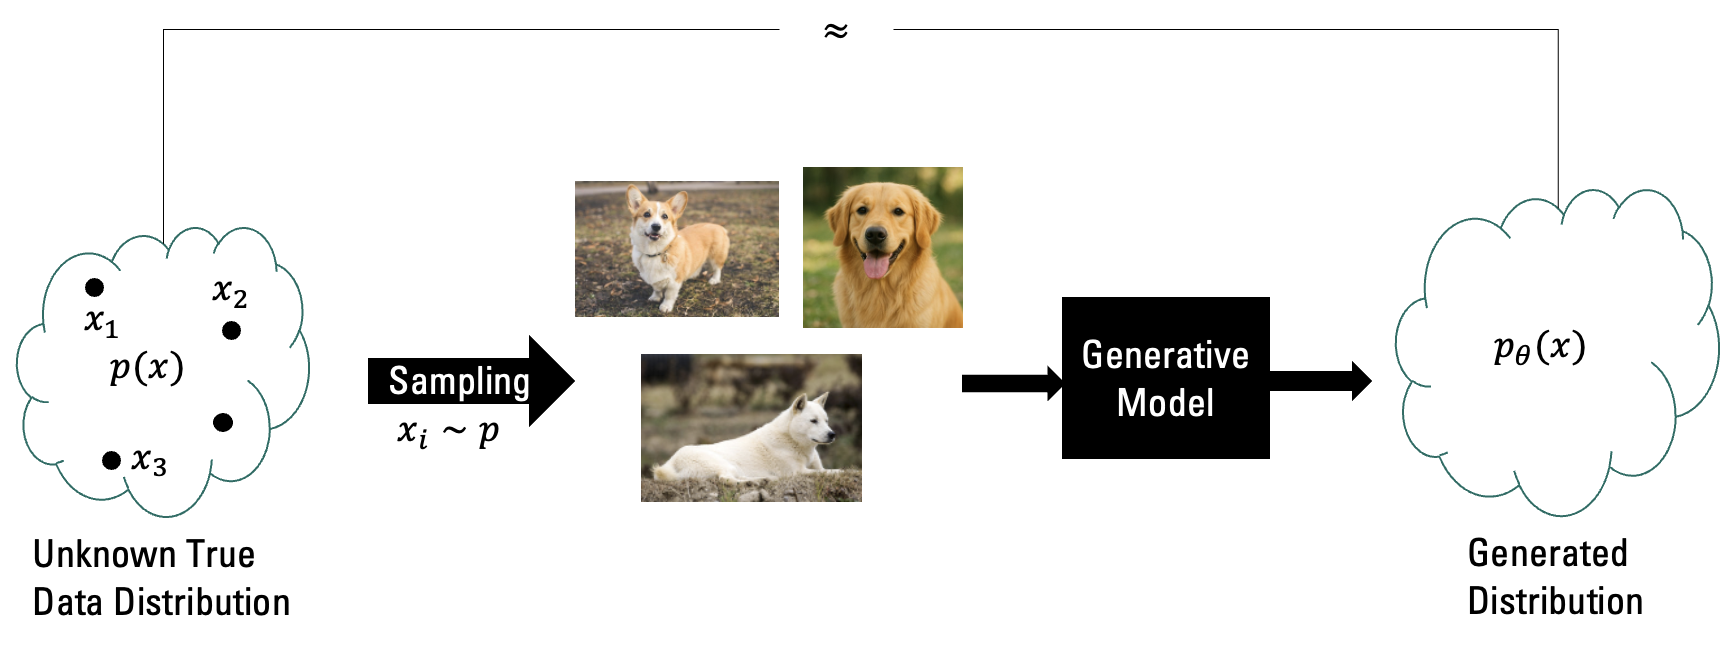
\includegraphics[width=1\linewidth]{figure/generative_model.png}
                \caption{Generative Model}
                \label{fig:generative_model}
            \end{figure}
			
			\note{The fundamental problem in generative modeling is that we have an unknown data distribution $p(x)$ that we want to learn. 
				  Even though we don't know the true distribution, we have access to samples from it, which we can use for training. 
				  Our goal is to design a generative model parameterised by theta that creates a distribution $p_theta(x)$ which approximates the true data distribution as closely as possible. 
				  This is essentially a density estimation problem where we learn to model the probability distribution of our training data. 
				  The key challenge is that we need to learn the entire distribution, not just make point predictions.}
		\end{frame}
    
        \begin{frame}{Constraints}
            \begin{itemize}
                \item Non-negativity: $$p_{\theta}(x) \geq 0 \quad \forall x$$
                \item Normalisation: $$\int p_{\theta}(x) dx = 1$$
            \end{itemize}
			
			\note{Since we're modeling probability distributions, we must satisfy two key constraints. 
				  First, non-negativity requires that all probabilities must be non-negative, which is relatively straightforward to enforce using positive functions. 
				  This constraint is not hard to match since we can use any kind of positive functions, such as exponentials or squared functions. 
				  Second, normalisation requires that the integral over all possible values must equal one, which is the constraint that makes computation challenging. 
				  This normalisation constraint is what drives many of the design choices in different generative model families. 
				  Different approaches handle this constraint in different ways: some compute the normalisation explicitly, others avoid it entirely, and some approximate it. 
				  The normalisation constant, also called the partition function, is often intractable for high-dimensional distributions. 
				  This intractability is one of the main reasons why we need sophisticated techniques like variational inference or adversarial training.}
        \end{frame}

        \begin{frame}{KL Divergence}
            Given $p(x)$, the true distribution the data actually follows, and $p_{\theta}(x)$, the approximate distribution,
            $$D_{\mathrm{KL}}(p \Vert p_{\theta})  = \mathbb{E}_{x \sim p(x)} [\log{\frac{p(x)}{p_{\theta} (x)}}] = \int p(x) \log{\frac{p(x)}{p_{\theta}(x)}} dx = H(p, p_{\theta}) - H(p) \geq 0$$
            measures the closeness of two distributions.
			
			\note{KL divergence is a crucial metric for measuring how close our learned distribution is to the true data distribution. 
				  It measures the expected log ratio between the two distributions, with a value of zero indicating perfect matching. 
				  The KL divergence can be decomposed into the cross-entropy minus the entropy of the true distribution, showing it's always non-negative. 
				  This metric naturally arises when we try to minimise the distance between distributions, which guides our training objectives. 
				  The KL divergence is asymmetric, meaning $D_{KL}(p \Vert q)$ is not equal to $D_KL(q \Vert p)$, which has important implications for training. 
				  When we minimise $D_{KL}(p \Vert p_theta)$, we're essentially doing maximum likelihood estimation, which is a fundamental statistical approach. 
				  The KL divergence is also related to other important metrics like the Jensen-Shannon divergence used in GANs. 
				  This connection between KL divergence and maximum likelihood is fundamental to understanding how most generative models are trained.}
        \end{frame}

        \begin{frame}{Training Objective}
            Training objective of the generative model is to find $\theta$ that minimises KL divergence. \\
            As $p(x)$ is not dependent on $\theta$,
            $$\hat{\theta} = \arg \underset{\theta}{\min} \: D_{\mathrm{KL}} (p \Vert p_{\theta}) = \arg \underset{\theta}{\max} \: \mathbb{E}_{x \sim p(x)} [\log{p_{\theta}(x)}]$$
            which is equivalent to maximum likelihood estimation (MLE). \\
            Loss function is defined as 
            $$\mathcal{L} (\theta) = - \mathbb{E}_{x \sim p(x)} [\log{p_{\theta} (x)}]$$ 
        
			\note{Our training objective is to find parameters theta that minimise the KL divergence between the true and learned distributions. 
				  Since the true distribution $p(x)$ doesn't depend on theta, minimising KL divergence is equivalent to maximising the expected log-likelihood of the data. 
				  This is exactly the maximum likelihood estimation principle, which is a fundamental statistical approach. 
				  The loss function is simply the negative log-likelihood, which we minimise during training. 
				  Maximum likelihood estimation is a principled approach that has strong theoretical guarantees under certain conditions. 
				  However, computing the exact likelihood is often intractable for complex models, which motivates various approximation techniques. 
				  Some models, like autoregressive models, can compute exact likelihoods efficiently. 
				  Other models, like VAEs, use lower bounds on the likelihood that can be computed efficiently. 
				  Still other models, like GANs, don't explicitly model likelihoods at all but match distributions through adversarial training. 
				  The choice of objective function fundamentally shapes how each model family is trained and what they can learn.}
		\end{frame}

        \begin{frame}{Taxonomy}
            \begin{figure}
                \centering
                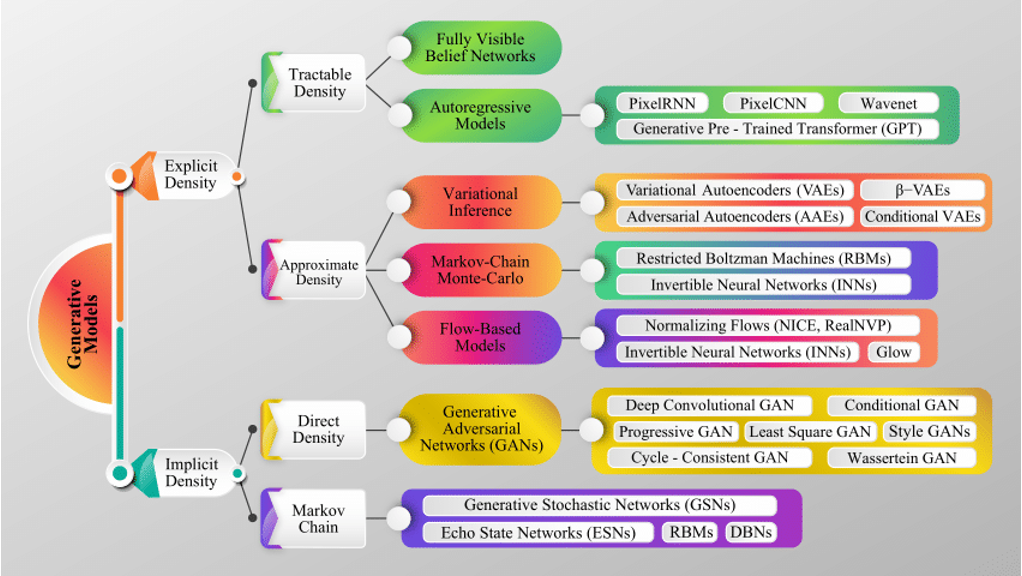
\includegraphics[width=0.7\linewidth]{figure/taxonomy.png}
                \caption{Taxonomy. Image from Çelik \& Eltawil (2024) – At the Dawn of Generative AI Era.}
                \label{fig:taxonomy}
            \end{figure}
			
			\note{Generative models can be organized into several families based on how they handle the normalization constraint. 
				  Explicit models directly compute likelihoods and can be further divided into factorized models like autoregressive models, latent variable models like VAEs, and invertible models like normalizing flows. 
				  Implicit models like GANs don't explicitly compute likelihoods but match distributions through adversarial training. 
				  Energy-based and score-based models work with unnormalized distributions and learn score functions instead. 
				  This taxonomy helps us understand the fundamental differences between approaches and their computational requirements.} 
		\end{frame}

    \section{Models}
        \subsection{Autoregressive Model (ARM)}
            \begin{frame}{Intuition}
                \begin{figure}
                    \centering
                    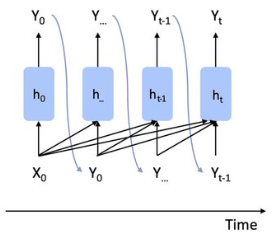
\includegraphics[width=0.45\linewidth]{figure/autoregressive.png}
                    \caption{Autoregressive model. Image from Mardikoraem et al. (2023) - Generative Models for Protein Sequence Modelling.}
                    \label{fig:autoregressive}                    
                \end{figure}
				
				\note{Autoregressive models are particularly well-suited for sequential data because they model the joint distribution as a product of conditional distributions. 
					  The key insight is that the output at each time step is fed back as input for the next time step, creating a natural dependency structure. 
					  This makes them perfect for tasks like language modeling, where each word depends on all previous words. 
					  The sequential nature allows us to break down complex joint distributions into simpler conditional probabilities. 
					  Autoregressive models factorize the joint distribution using the chain rule of probability, expressing it as a product of conditional probabilities. 
					  Each conditional probability depends only on the previous elements in the sequence, making the computation tractable. 
					  This approach is very powerful for sequences like text, audio, and time series data.  
					  The autoregressive structure allows for efficient training using teacher forcing, where ground truth inputs are used during training. 
					  However, sampling requires sequential generation, which can be slow for long sequences.}
            \end{frame}

            \begin{frame}{Objective}
                ARM factorises the joint distribution using the chain rule 
                $$p_{\theta} (x) = \prod_{t = 1}^{T} p_{\theta} (x_{t} \mid x_{<t}) \; \badgeT$$
                for sequence $x = (x_{1}, \cdots, x_{T})$. \\
                Loss function is
                $$\mathcal{L} (\theta) = -\sum_{t=1}^{T} \log{p_{\theta} (x_{t} \mid x_{<t})} \; \badgeT$$
            
				\note{Autoregressive models factorize the joint distribution using the chain rule of probability, expressing it as a product of conditional probabilities. 
					  Each conditional probability depends only on the previous elements in the sequence, making the computation tractable. 
					  The loss function is simply the sum of negative log-likelihoods of each conditional probability, which can be computed exactly. 
					  This tractability makes training straightforward, though sampling requires sequential generation which can be slow. 
					  The objective is to maximize the log-likelihood of the entire sequence, which decomposes into a sum over time steps.}
			\end{frame}

            \begin{frame}{Architecture}
                \begin{figure}
                    \centering
                    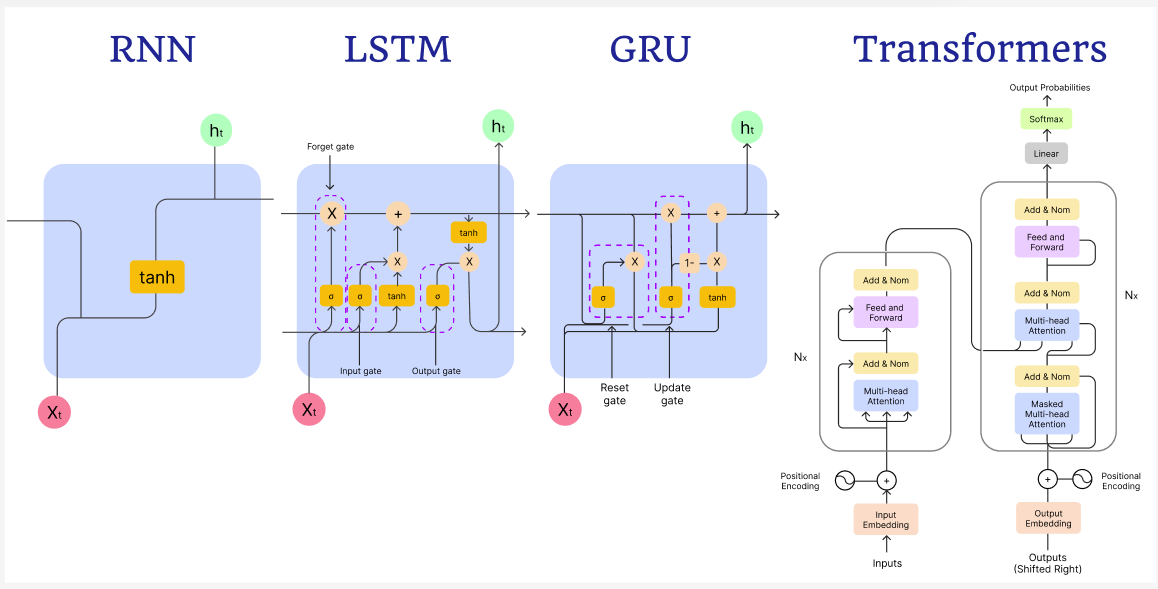
\includegraphics[width=0.8\linewidth]{figure/ar_models.png}
                    \caption{Examples of AR models. Image from \url{https://code-b.dev/blog/autoregressive-language-model}.}
                    \label{fig:ar_models}
                \end{figure}
				
				\note{It's important to note that not all transformers are autoregressive - the key is in how they're used. 
				For a transformer to be autoregressive, we need to factorize the data likelihood from left to right and enforce a causal mask. 
				This causal mask ensures that each position can only attend to previous tokens, not future ones. 
				Examples of autoregressive models include GPT, PixelCNN, and WaveNet, which all use this left-to-right factorization. 
				The transformer architecture is very flexible and can be used for both autoregressive and non-autoregressive tasks. 
				For autoregressive language modeling, the decoder-only transformer with causal masking is standard. 
				The causal mask prevents information leakage from future tokens, ensuring valid probability distributions. 
				This architecture allows the model to efficiently process sequences while maintaining the autoregressive property. 
				The attention mechanism enables the model to capture long-range dependencies while respecting the causal constraint.}
            \end{frame}
        
        \subsection{Variational Autoencoder (VAE)}
            \begin{frame}{Intuition}
                \begin{figure}
                    \centering
                    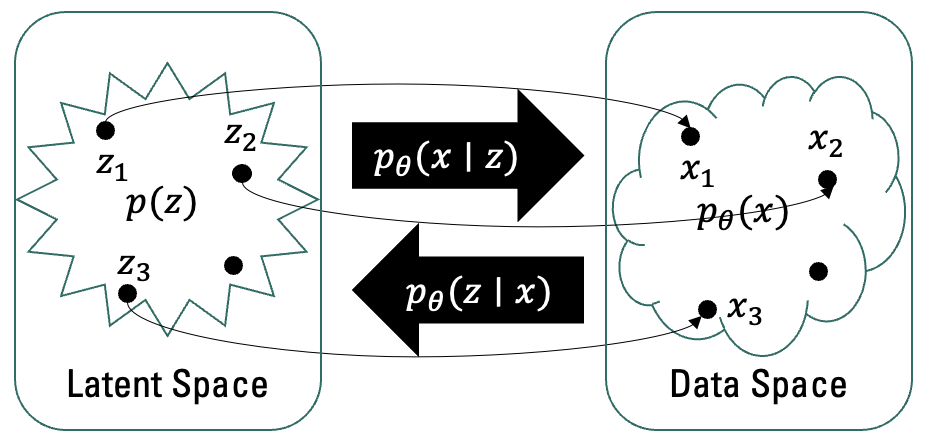
\includegraphics[width=0.8\linewidth]{figure/latent_variables.png}
                    \caption{Latent \& Data Space}
                    \label{fig:latent_var}
                \end{figure}
				
				\note{Properties of data distribution $p(x)$ are unknown, but some samples from $p(x)$ can be accessed. 
					  VAEs introduce the concept of latent variables, which are vectors in a lower-dimensional continuous space that capture underlying factors of variation in the data. 
					  Since $p(x)$ and $p(z)$ reside in different spaces, a mapping is required to connect them. 
					  The posterior distribution $p_{\theta}(z \mid x)$ is the mapping from $p(x)$ to $p(z)$, which indicates the probability of latent vector z generated by particular data $x$. 
					  The likelihood distribution $p_{\theta}(x \mid z)$ is the mapping from $p(z)$ to $p(x)$, which gives the probability of reconstructing x from latent vector $z$. 
					  If latent vectors are sampled from the posterior distribution, those are likely to have been generated by the original distribution $p(x)$. 
					  The encoder takes data $x$ and produces a latent code $z$, while the decoder takes $z$ and reconstructs $x$. 
					  Unlike regular autoencoders which represent data as a single point in latent space, VAEs represent data as a Gaussian distribution. 
					  This probabilistic representation allows for smooth interpolation and generation of new data by sampling from the latent space. 
					  The key insight is that by learning a meaningful latent representation, we can generate new data points by sampling from the latent distribution and decoding them.}
            \end{frame}

            \begin{frame}{Definition}
                \begin{block}{Joint distribution}
                    $p(x, z) = p(x \mid z) p(z)$
                \end{block}

                \begin{block}{Marginal likelihood (Evidence)}
                    $p(x) = \int p(x, z) dz$ \\
                \end{block}

                \begin{block}{Posterior}
                    $p(z \mid x) = \frac{p(z) p (x \mid z)}{p(x)}$ \\
                \end{block}

                \begin{block}{Jensen's Inequality}
                    Let $f$ be a convex function and $X$ a random variable, then $f(\mathbb{E} [X]) \leq \mathbb{E} [f(x)]$. \\
                    Inequality reverses for the concave function.
                \end{block}
				
				\note{The joint distribution $p(x, z)$ factors into the product of the prior $p(z)$ and the likelihood $p(x \mid z)$, representing the complete generative process. 
					  The marginal likelihood, also called the evidence $p_{\theta}(x)$, is the integral over all possible latent values $z$, which is typically intractable for complex models. 
					  This intractability is the fundamental challenge that motivates the use of variational inference in VAEs. 
					  The posterior distribution $p_{\theta}(z \mid x)$ tells us which latent values likely generated each data point, but computing it requires the intractable marginal likelihood. 
					  Jensen's inequality is crucial for deriving a lower bound on the log-likelihood that we can actually optimize. 
					  For convex functions, Jensen's inequality states that the function of the expectation is less than or equal to the expectation of the function. 
					  This inequality allows us to move the log inside the expectation, creating a lower bound that we can compute. 
					  The logarithm is a concave function, so we need to be careful about the direction of the inequality. 
					  By applying Jensen's inequality to the log-likelihood, we can derive the Evidence Lower Bound, or ELBO, which provides a tractable objective for training. 
					  This lower bound will be our surrogate objective that we can optimize using gradient descent.}
            \end{frame}

            \begin{frame}{Assumptions}
                \begin{itemize}
                    \item Prior: \\
                    Set $p(z) = \mathcal{N} (0, I) \; \badgeT$  \; to make sampling and regularisation easy.
                    \item Likelihood: \\
                    Set $p_{\theta}(x \mid z)=\mathcal{N}(\mu_{\theta}(z), \sigma_{\theta}^{2}(z)I) \; \badgeT$ parameterised by the decoder.
                    \item Posterior: \\
                    $p_{\theta} (z \mid x) \; \badgeI$ is intractable. \\
                    Introduce an approximate posterior $q_{\phi} (z \mid x) = \mathcal{N} (\mu_{\phi} (x), \sigma_{\phi}^{2} (x) I) \; \badgeA$ parameterised by the encoder.
                \end{itemize}
				
				\note{To make VAEs tractable, we make specific distributional assumptions about the prior, likelihood, and posterior. 
					  The prior $p(z)$ is set to a standard Gaussian distribution $\mathcal{N}(0, I)$, which is a design choice that makes sampling easy and provides regularization. 
					  This choice is reasonable because it assumes latent codes should be distributed around zero with unit variance, encouraging the model to learn compact representations. 
					  The likelihood $p_{\theta}(x \mid z)$ is also assumed to be Gaussian, parameterized by a decoder network that outputs mean and variance. 
					  This Gaussian assumption allows us to compute the reconstruction loss efficiently while still being expressive enough to model complex data. 
					  The true posterior $p_{\theta}(z \mid x)$ is intractable because it requires computing the marginal likelihood, which involves an intractable integral. 
					  Instead, we introduce an approximate posterior $q_{\phi}(z \mid x)$, also Gaussian, parameterized by an encoder network. 
					  The encoder network takes input data $x$ and outputs parameters $\mu_{\phi}(x)$ and $\sigma_{\phi}(x)$ that define the approximate posterior distribution. 
					  These Gaussian assumptions allow for efficient computation while still being expressive enough to model complex data distributions. 
					  The key insight is that we can approximate the intractable posterior with a simpler distribution that we can learn and sample from efficiently.}
            \end{frame}

            \begin{frame}{Evidence Lower Bound (ELBO)}
                \small
                \begin{align*}
                    \log{p_{\theta} (x)} & = \log{\int p_{\theta} (x, z) dz} & \text{(Definition of marginal likelihood)} \\ 
                    & = \log{\int p_{\theta} (x, z) \frac{q_{\phi} (z \mid x)}{q_{\phi} (z \mid x)} dz} \\
                    & = \log{\mathbb{E}_{q_{\phi} (z \mid x)}} \frac{p_{\theta} (x, z)}{q_{\phi} (z \mid x)} & \text{(Definition of expectation)} \\ 
                    & \geq \mathbb{E}_{q_{\phi}(z \mid x)} [\log{\frac{p_{\theta} (x \mid z) p(z)}{q_{\phi} (z \mid x)}}] & \text{(Jensen's inequality)} \\
                    & = \underbrace{\mathbb{E}_{q_{\phi}(z \mid x)} [\log{p_{\theta} (x \mid z)}]}_{\mathcal{L}_{\mathrm{rec}} \; \badgeA} - \underbrace{D_{KL}(q_{\phi}(z \mid x) \Vert p(z))}_{\mathcal{L}_{\mathrm{reg}} \; \badgeT} & \text{(Definition of KL Divergence)} 
                \end{align*}
				
				\note{The ELBO derivation starts with the log-likelihood, which we want to maximize but cannot compute directly. 
					  We introduce the approximate posterior $q_{\phi}(z \mid x)$ by multiplying and dividing by it, which doesn't change the value but allows us to rewrite the expression. 
					  This trick converts the integral into an expectation over the approximate posterior, which we can approximate using Monte Carlo sampling. 
					  We then apply Jensen's inequality to the logarithm, which is a concave function, to obtain a lower bound on the log-likelihood. 
					  The ELBO decomposes into two terms: a reconstruction term and a regularization term. 
					  The first term is the reconstruction term $L_{rec}$, which encourages the decoder to reconstruct data well from latent samples. 
					  This term measures how well the model can reconstruct the input data $x$ given latent samples $z$ from the approximate posterior. 
					  The second term is the prior matching term $L_{reg}$, which is the KL divergence between the approximate posterior and the prior. 
					  This term encourages the encoder's distribution $q_{\phi}(z \mid x)$ to be close to the prior $p(z)$ and prevents the encoder from collapsing into a trivial deterministic mapping. 
					  The KL divergence acts as a regularizer that prevents overfitting and ensures the latent space follows our prior assumptions.}
            \end{frame}

            \begin{frame}{Monte Carlo Method}
                Monte Carlo method is a way to approximate expectations (integrals) using random samples. \\
                Integral is often too complicated to compute exactly. \\
                Instead, draw samples $x^{(1)}, \cdots, x^{(N)} \sim p(x)$. \\
                If $N$ is large enough, by the law of large numbers,
                $$\mathbb{E}_{x \sim p(x)} [f(x)] = \int f(x) p(x) dx \approx \frac{1}{N} \sum_{i = 1}^{N} f(x^{(i)})$$
				
				\note{The Monte Carlo method is a powerful technique for approximating expectations that would otherwise be intractable. 
					  The key idea is that we can approximate integrals by drawing random samples and computing averages. 
					  This works because of the law of large numbers, which guarantees that as we draw more samples, our approximation gets better. 
					  In the context of VAEs, we use Monte Carlo sampling to approximate the expectation over the approximate posterior during training. 
					  Many integrals in machine learning, especially those involving high-dimensional spaces, are too complicated to compute exactly. 
					  Instead of computing the integral directly, we draw samples $x^(1)$ through $x^(N)$ from the distribution $p(x)$, and then compute the average of the function values at these samples.}
            \end{frame}

            \begin{frame}{Objective}
                The objective of VAE is equivalent to maximising the ELBO. \\
                By the Monte-Carlo approximation, 
                $$\mathbb{E}_{z \sim q_{\phi} (z \mid x)} [\log{f(z)}] \approx \frac{1}{L} \sum_{l = 1}^{L} f(z^{(l)}) \; \badgeT$$ 
                where $z^{(l)} \sim q_{\phi} (z \mid x)$ and $f(z) = \log{\frac{p_{\theta} (x, z)}{q_{\phi} (z \mid x)}}$.
            
				\note{The VAE training objective is to maximize the ELBO, which provides a lower bound on the log-likelihood. 
					  Since the ELBO involves expectations that are intractable, we use Monte Carlo approximation to estimate them. 
					  Instead of computing the exact expectation over the approximate posterior, we draw L samples from $q_{\phi}(z \mid x)$ and compute the average. 
					  The function $f(z)$ we're taking the expectation of is the log-ratio of the joint distribution to the approximate posterior. 
					  This log-ratio can be decomposed into the log-likelihood minus the log of the approximate posterior, which simplifies the computation. 
					  In practice, we typically use just one sample ($L = 1$) per data point during training, which is surprisingly effective. 
					  The key challenge is that directly sampling from $q_{\phi}(z \mid x)$ is not differentiable, so we cannot backpropagate through the sampling process. 
					  This is where the reparameterization trick becomes essential for making VAE training work with stochastic gradient descent. 
					  The reparameterization trick allows us to separate the stochastic part from the deterministic part, making the sampling process differentiable. 
					  Without this trick, we would not be able to use gradient-based optimization methods to train the encoder and decoder networks.}
			\end{frame}

            \begin{frame}{Reparameterisation Trick}
                Samples from a Gaussian distribution $z \sim \mathcal{N} (\mu_{\phi} (x), \sigma_{\phi}^{2} (x) I)$ can be rewritten as a combination of a deterministic function and a noise variable 
                $$z = \mu_{\phi} (x) + \sigma_{\phi} (x) \odot \epsilon$$ 
                where $\epsilon \sim \mathcal{N} (0, 1)$.
				
				\note{The reparameterization trick is essential for making VAE training work with stochastic gradient descent. 
					  The problem is that sampling directly from $q_{\phi}(z \mid x)$ is a stochastic operation that cannot be backpropagated through. 
					  Instead of sampling z directly from the Gaussian distribution, we reparameterize by separating the sampling into two parts: a deterministic function of parameters, and independent noise. 
					  For a Gaussian distribution, we can rewrite $z$ as $\mu_{\phi}(x)$ plus $\sigma_{\phi}(x)$ times epsilon, where epsilon is sampled from a standard Gaussian. 
					  The key insight is that epsilon is independent of the parameters phi, so we can move the gradient operator inside the expectation. 
					  This means that the expectation is now taken over epsilon, which is independent of phi, allowing us to backpropagate through the deterministic parts. 
					  The gradient of the expectation with respect to phi can now be computed as the expectation of the gradient, which we can estimate using Monte Carlo sampling. 
					  This trick enables end-to-end training of the VAE using standard backpropagation and stochastic gradient descent.}
            \end{frame}

            \begin{frame}{Architecture}
                \begin{figure}
                    \centering
                    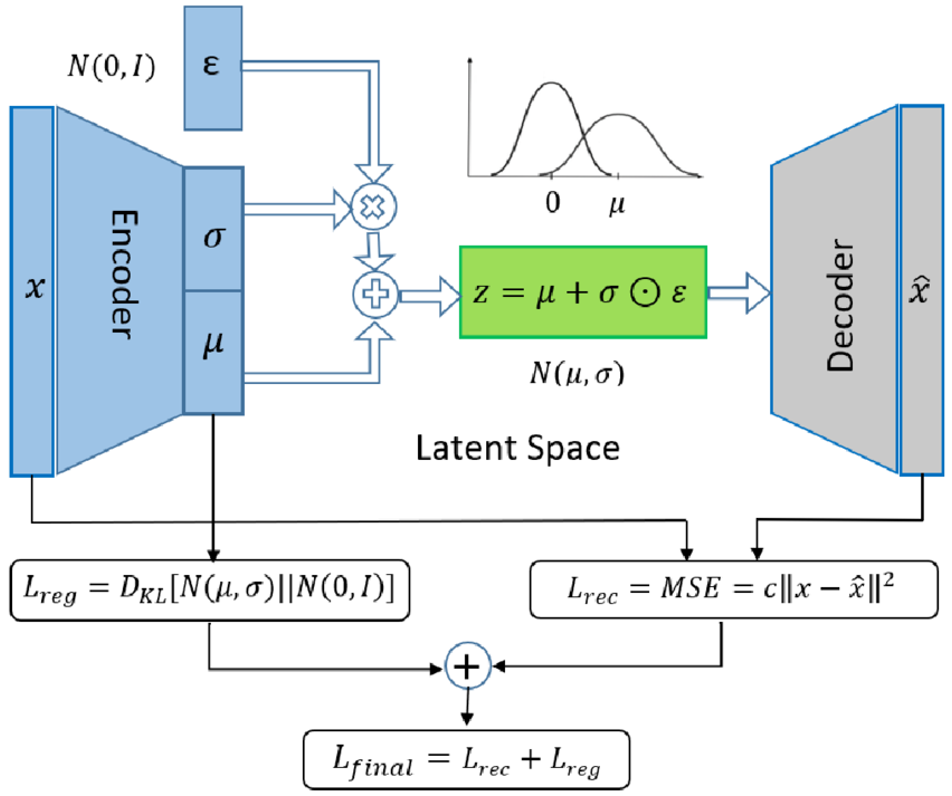
\includegraphics[width=0.4\linewidth]{figure/vae.png}
                    \caption{VAE. Image from Puchalski \& Komorska (2023) – Generative Modelling of Vibration Signals in Machine Maintenance.}
                    \label{fig:vae}
                \end{figure}
				
				\note{The VAE architecture consists of two main components: an encoder network and a decoder network. 
					  The encoder takes input data $x$ and produces parameters $\mu_{\phi}(x)$ and $\sigma_{\phi}(x)$ that define the approximate posterior distribution $q_{\phi}(z \mid x)$. 
					  The encoder converts the input into a probability distribution, specifically chosen to be a Gaussian, unlike regular autoencoders which output deterministic codes. 
					  From the Gaussian distribution in the latent space, we sample points at random using the reparameterization trick. 
					  The decoder network then takes these sampled latent codes z and reconstructs the input data x, parameterizing the likelihood distribution $p_{\theta}(x \mid z)$. 
					  During training, we encode data to get latent distributions, sample from these distributions using the reparameterization trick, and decode to reconstruct the input. 
					  The loss function combines a reconstruction loss, which measures how well the decoder reconstructs the input, and a KL divergence term, which regularizes the latent distribution. 
					  This architecture enables smooth interpolation in latent space and generation of new data by sampling from the prior $p(z)$ and decoding. 
					  The key advantage of this probabilistic approach is that it learns a meaningful latent representation that captures the underlying structure of the data. 
					  By forcing the latent codes to follow a Gaussian distribution, the encoder is forced to arrange codes efficiently, and the decoder sees training samples across the whole region, preventing holes in the latent space.}
            \end{frame}

        \subsection{Normalising Flow}
            \begin{frame}{Intuition}
                \begin{figure}
                    \centering
                    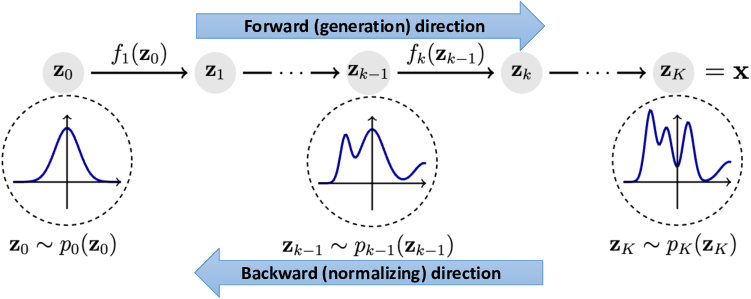
\includegraphics[width=0.7\linewidth]{figure/flow.png}
                    \caption{Normalising flow. Image from Shen \& Shen (2023) – PSRFlo.}
                    \label{fig:normalising_flow}
                \end{figure}
				
				\note{Normalizing flows learn an invertible transformation between a simple, tractable base distribution and a complex data distribution. 
					  Let $f_{\theta}$ be a bijection that maps model data x to the image of a latent variable $z$, so that $x = f_{\theta}(z)$ and $z = f_{\theta}^{-1}(x)$. 
					  The idea is to start with a simple distribution like a standard Gaussian $p_{Z}$ and apply learned invertible functions that gradually make it more complex. 
					  As $f_{\theta}$ is invertible and differentiable, exact data log-likelihoods can be computed using the change of variables formula. 
					  This yields a maximum-likelihood training objective that is tractable and does not rely on adversarial training or approximate posteriors. 
					  A standard normalizing flow commits to explicit, finite-depth, invertible maps. 
					  Each transformation in the flow must be invertible and have a tractable Jacobian determinant, which allows us to compute the exact likelihood. 
					  This approach gives us exact likelihoods and fast sampling, but requires careful design of the transformations. 
					  The key challenge is designing transformations that are both expressive and computationally efficient, especially for the Jacobian determinant computation.}
            \end{frame}

            \begin{frame}{Flow (Discrete)}
                Let $f_{\theta}$ be invertible, differential map where $z = f_{\theta}^{-1}(x)$. \\
                $f_{\theta} = f_{K} \circ f_{K - 1} \circ \cdots \circ f_{1}$ where $f_{k}$ is chosen such that the Jacobian determinant is cheap.
				
				\note{In discrete normalizing flows, we compose multiple invertible transformations to create complex distributions. 
					  The overall transformation $f_{\theta}$ is the composition of $K$ simpler transformations, each chosen to have a cheap-to-compute Jacobian determinant. 
					  Each transformation $f_{k}$ must be invertible and differentiable, ensuring that the overall composition is also invertible and differentiable. 
					  The key challenge is designing transformations that are both expressive and computationally efficient for computing Jacobian determinants. 
					  Computing the determinant of n times n Jacobian matrices is expensive in general, so we choose transformations that result in special matrix structures. 
					  Common choices include triangular matrices, diagonal matrices, or other structures that allow efficient determinant computation. 
					  Coupling layers and autoregressive flows are popular choices that ensure invertibility while allowing flexible transformations.}
            \end{frame}

            \begin{frame}{Change of Variables Theorem}
                Suppose $z \in \mathbb{R}^{d}$, and $x = f(z)$ with $f : \mathbb{R}^{d} \to \mathbb{R}^{d}$ a diffeomorphism.
                $$p_{X}(x) = p_{Z}(f_{\theta}^{-1}(x)) \lvert \det{J_{f_{\theta}^{-1}}(x)} \rvert = p_{Z}(z) \lvert \frac{1}{\det{J_{f_{\theta}}(z)}} \rvert$$
				
				\note{The change of variables theorem is fundamental to normalizing flows, telling us how probability densities transform under invertible maps. 
					  When we apply an invertible function $f$, the density in the output space $p_{X}(x)$ is related to the input density $p_{Z}(z)$ by the absolute value of the Jacobian determinant. 
					  The Jacobian determinant captures how the transformation stretches or compresses volumes in space. 
					  If the transformation expands volumes, the density decreases, and if it contracts volumes, the density increases. 
					  The absolute value ensures that the probability density remains non-negative, regardless of the sign of the determinant. 
					  For the inverse transformation, we can express the density in terms of the forward transformation's Jacobian. 
					  The determinant of the inverse Jacobian equals one over the determinant of the forward Jacobian, which is useful for computation. 
					  This theorem allows us to compute exact likelihoods in the data space from the simple base distribution. 
					  The key requirement is that $f$ must be a diffeomorphism, meaning it is invertible, differentiable, and has a differentiable inverse.}
            \end{frame}

            \begin{frame}{Objective}
                By the change of variables theorem, 
                $$\log{p_{X} (x)} = \log{p_{Z}(f_{\theta}^{-1}(x))} - \log{\lvert \det J_{f_{\theta}}(f_{\theta}^{-1}(x)) \rvert}$$ \\
                Since $f_{\theta} = f_{K} \circ f_{K - 1} \circ \cdots \circ f_{1}$, starting with the data space density $p_{Z_{0}}(z_{0}) = p_{X}(x)$, \\ 
                the first transformation $f_{1}: z_{0} \mapsto z_{1}$ gives $\log{p_{Z_0}(z_0)} = \log{p_{Z_1}(z_1)} - \log{\lvert \det{J_{f_1}(z_0)} \rvert}.$ \\
                The second transformation $f_{2}: z_{1} \mapsto z_{2}$ gives $\log{p_{Z_1}(z_1)} = \log{p_{Z_2}(z_2)} - \log{\lvert \det{J_{f_2}(z_1)} \rvert}.$ \\
                After repeating for all $K$ transformations with $z_{0} = x$ and $z_{k} = z$,
                $$\log{p_{X} (x)} = \log{p_{Z} (z)} - \sum_{k = 1}^{K} \log{\lvert \det{J_{f_{k}} (z_{k - 1})} \rvert} \; \badgeT$$
				
				\note{For normalizing flows, the log-likelihood can be computed exactly using the change of variables theorem. 
					  The log-likelihood equals the log-likelihood in the base space minus the sum of log absolute Jacobian determinants. 
					  Each transformation in the flow contributes a correction term that accounts for how it changes the volume of the space. 
					  This sum accumulates the volume changes from each transformation in the flow. 
					  Starting with the data space density $p_{X}(x)$, we apply the first transformation $f_{1}$ to get $z_{1}$, which requires computing the Jacobian determinant of $f_{1}$. 
					  We then apply the second transformation $f_{2}$ to get $z_{2}$, accumulating another Jacobian determinant term. 
					  This process continues for all $K$ transformations until we reach the base space density $p_{Z}(z)$. 
					  The key advantage is that we get exact likelihoods, unlike VAEs which have a variational gap, and we can optimize this directly using maximum likelihood.}
			\end{frame}

        \subsection{Flow Matching}
            \begin{frame}{Intuition}
                \begin{figure}
                    \centering
                    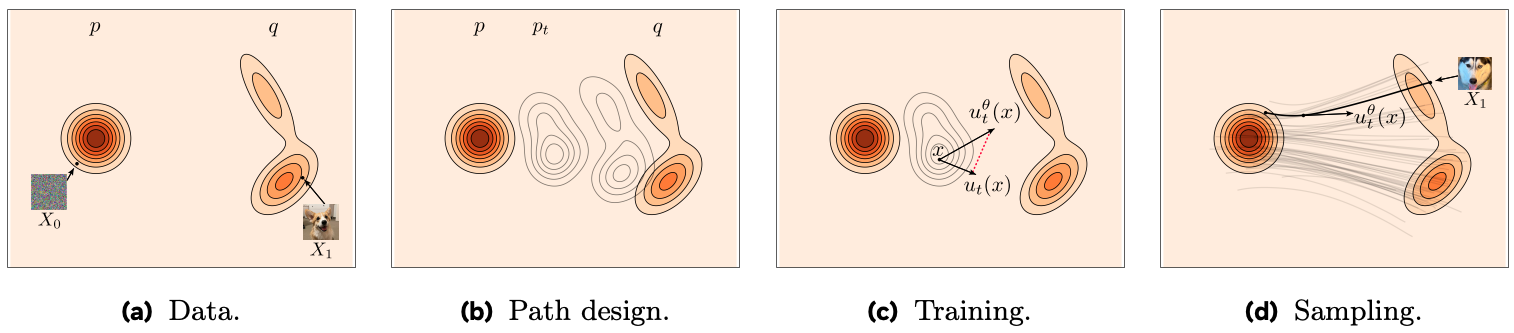
\includegraphics[width=1\linewidth]{figure/flow_matching.png}
                    \caption{Flow matching. Image from Lipman et al. (2024) - Flow Matching Guide and Code.}
                    \label{fig:flow_matching}
                \end{figure}
				
				\note{Diffusion models work by gradually adding noise to data through a multi-step process until it becomes a standard normal distribution. 
					  Starting from a clean image, noise is added iteratively until the image becomes pure noise following a standard normal distribution. 
					  Since the standard normal distribution is known, we can sample from it easily. 
					  Then, by tracing back or denoising through intermediate steps, we can recover the clean image. 
					  Flow matching generalizes this discrete diffusion process to a continuous flow. 
					  Let $p_{0}$ be the standard normal distribution and $p_{1}$ be the data distribution that we want to learn. 
					  The key insight is that $p_{0}$ can morph directly to $p_{1}$ without explicitly defining intermediate discrete steps. 
					  However, $p_{1}$ is unknown and we only have a finite number of samples available. 
					  Hence, we define an approximate distribution q which is generated by a mixture of Gaussian distributions at sample points. 
					  Flow matching is the modeling of the morphism from $p_{0}$ to $q$, learning a continuous velocity field that transports the noise distribution to the data distribution.}					  
            \end{frame}

            \begin{frame}{Flow (Continuous)}
                ODE $\frac{d}{dt} \psi_{t} (x) = u_{t} (\psi_{t} (x))$ where $\psi_{t} = \psi(t, x)$ and $\psi_{0}(x) = x$ describes how a point in space moves over time under a velocity rule. \\
                $\psi_{t} \in \mathbb{R}^{d}$ is a solution to the ODE called a trajectory, which represents the position of a particle at time $t$. \\
                $u_{t}(x) \in \mathbb{R}^{d}$ is a vector field that gives the velocity at location $x$ at time $t$.
            
				\note{In continuous flows, we describe the evolution using an ordinary differential equation or ODE. 
					  The ODE defines a velocity field $u_{t}(x)$ that tells us how points move through space over time. 
					  The flow $\psi_{t}(x)$ is the solution to this ODE, representing the trajectory of a point starting at position $x$. 
					  At time $t = 0$, the flow starts at the initial position, so $\psi_{0}(x) = x$. 
					  As time progresses, each point follows a trajectory determined by the velocity field at its current location. 
					  The velocity field $u_{t}(x)$ is learned by a neural network, parameterized by theta, allowing us to model complex transformations. 
					  This continuous formulation is more flexible than discrete normalizing flows, as it allows for smoother paths between distributions. 
					  The key advantage is that we can learn the velocity field directly, rather than composing many discrete transformations. }
			\end{frame}

            \begin{frame}{Definition}
                \begin{block}{Probability Path}
                    The velocity field $u_{t}$ generates the probability path $p_{t}$ if its flow $\psi_{t}$ satisfies $X_{t} = \psi_{t}(X_{0}) \sim p_{t}$ for $X_{0} \sim p_{0}$.
                \end{block}
            
                \begin{block}{Push Forward}
                    ODE induces a push-forward of distributions $p_{t} = (\psi_{t})_{\#} p_{0}$ meaning if sample $x_{0} \sim p_{0}$ is pushed through the flow $\psi_{t}$, the resulting distribution is $p_{t}$. \\
                    By the change of variables theorem, if $y = \psi_{t} (x)$, then $p_{t} (y) = p_{0} (\psi_{t}^{-1} (y)) \lvert \det \frac{\partial}{\partial y} \psi_{t}^{-1} (y) \rvert$.
                \end{block}
            
                \begin{block}{Continuity Equation}
                    The evolution of probability densities under a velocity field is governed by the continuity equation $\frac{\partial}{\partial t}p_{t}(x) + \nabla \cdot (p_{t}(x) u_{t}(x)) = 0$.
                \end{block}
				
				\note{The formal definitions in flow matching establish the mathematical framework for continuous transformations. 
					  A probability path $p_{t}$ is generated by a velocity field $u_{t}$ if samples evolved through the flow $\psi_{t}$ follow that path. 
					  This means that if we start with samples from $p_{0}$ and evolve them according to the flow, they will be distributed according to $p_{t}$ at time $t$. 
					  The push-forward operation describes how distributions transform under the flow, moving from simple to complex. 
					  When we push a sample $x_{0}$ through the flow $\psi_{t}$, we get a new sample $y = \psi_{t}(x_{0})$, and the distribution of these transformed samples is $p_{t}$. 
					  The change of variables theorem tells us how the probability density transforms under this push-forward operation. 
					  The continuity equation governs how probability densities evolve over time, ensuring conservation of probability mass. 
					  This equation ensures that probability is neither created nor destroyed during the flow, only transported. 
					  The continuity equation is a fundamental constraint that any valid probability flow must satisfy.} 
            \end{frame}

            \begin{frame}{Assumptions}
                True marginal velocity field $u_{t}(x) \; \badgeI $ that takes $p_{0} \to p_{1}$ is intractable. \\
                Construct an interpolation between samples of $p_{0}$ and $p_{1}$. \\
                For two endpoints $x_{0} \sim p_{0}$ and $x_{1} \sim p_{1}$, using a linear interpolation, $x_{t} = (1 - t) x_{0} + t x_{1}$. \\
                If $x_{0}, x_{1}$ are fixed, then $x_{t}$ is deterministic. \\
                Hence, the random variable $X_{t}$ conditioned on a pair $(x_{0}, x_{1})$ has distribution $p_{t} (x \mid x_{0}, x_{1}) = \delta (x - ((1 - t) x_{0} + t x_{1}))$. \\
                Furthermore, $\frac{d}{dt} x_{t} = x_{1} - x_{0} = \frac{x_{1} - x_{t}}{1 - t} = u_{t}^{*} (x_{t} \mid x_{1}) \; \badgeT$ becomes a tractable conditional target velocity. 
				
				\note{The true marginal velocity field that takes us from noise $p_{0}$ to data $p_{1}$ is intractable to compute exactly. 
					  Instead of trying to learn this intractable marginal velocity field, we construct conditional velocity fields by interpolating between pairs of data points and noise samples. 
					  For each pair consisting of a noise sample $x_{0}$ from $p_{0}$ and a data sample $x_{1}$ from $p_{1}$, we use simple linear interpolation to create a path. 
					  The interpolated path is $x_{t} = (1 - t) x_{0} + t x_{1}$, which smoothly connects the noise sample to the data sample. 
					  If $x_{0}$ and $x_{1}$ are fixed, then $x_{t}$ is deterministic, making the path easy to compute. 
					  The conditional probability path $p_{t}(x \mid x_{0}, x_{1})$ is a delta function centered on the interpolated point, since the path is deterministic. 
					  The velocity along this path is simply the derivative with respect to time, which is $x_{1} - x_{0}$. 
					  This conditional velocity $u_{t} * (x_{t} \mid x_{1})$ is tractable and can be computed exactly for each pair of samples. 
					  The key insight is that optimizing with respect to this conditional velocity gives the same gradients as optimizing with respect to the intractable marginal velocity. 
					  This allows us to train the model using tractable conditional paths while achieving the same result as if we had used the intractable marginal paths.}
            \end{frame}
            
            \begin{frame}{Objective}
                The objective of flow matching is to train a model $u_{\theta} (x, t)$ by minimising MSE loss
                $$\mathcal{L}_{\mathrm{FM}} (\theta) = \mathbb{E}[\Vert u_{\theta}(x_{t}, t) - u_{t} (x_{t}) \Vert^{2}] \; \badgeI$$
                As the true marginal velocity field is intractable, use the conditional target velocity field instead, i.e.
                $$\mathcal{L}_{\mathrm{CFM}} (\theta) = \mathbb{E}[\Vert u_{\theta}(x_{t}, t) - u_{t}^{*} (x_{t} \mid x_{1}) \Vert^{2}] \; \badgeT$$
                Using conditional target velocity is valid because optimisation with respect to $\theta$ yields $\nabla_{\theta} \mathcal{L}_{\mathrm{FM}} = \nabla_{\theta} \mathcal{L}_{\mathrm{CFM}}$.
            
				\note{The flow matching objective trains a neural network $v_{\theta}(x, t)$ to predict the velocity field at any point and time. 
					  The ideal objective would minimize the difference to the true marginal velocity $u_{t}(x)$, but this is intractable. 
					  Instead, we use the conditional flow matching objective, which uses the conditional velocity field $u_{t} * (x_{t} \mid x_{1})$ as the target. 
					  The conditional flow matching loss is the expected squared error between the predicted velocity and the conditional target velocity. 
					  The expectation is taken over time $t$ sampled uniformly, data samples $x_{1}$ from $q(x_{1})$, and interpolated points $x_{t}$ from $p_{t}(x \mid x_{0}, x_{1})$. 
					  The key theoretical result is that optimizing the conditional objective gives the same gradients as optimizing the marginal objective. 
					  This means that optimizing $\mathcal{L}_{CFM}$ with respect to theta yields the same result as optimizing $\mathcal{L}_{FM}$, even though $\mathcal{L}_{FM}$ is intractable. 
					  This equivalence allows us to train the model using tractable conditional paths while achieving optimal performance. 
					  The conditional paths are defined on a per-sample basis, making them completely tractable and easy to compute. 
					  This formulation is much simpler than trying to work with the intractable marginal paths directly, while maintaining the same theoretical guarantees.}
			\end{frame}

        \subsection{Energy-Based Model (EBM)}
            \begin{frame}{Intuition}
                \begin{figure}
                    \centering
                    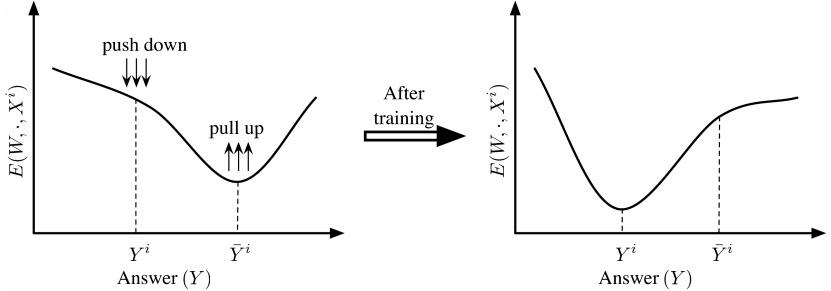
\includegraphics[width=0.8\linewidth]{figure/ebm.png}
                    \caption{Energy-based model.}
                    \label{fig:ebm}
                \end{figure}
				
				\note{Energy-based models define probability distributions through an energy function, where lower energy corresponds to higher probability. 
					  This framework is very flexible because we can use any function as an energy, without constraints like invertibility or specific architectures. 
					  The energy function naturally connects to physics, where systems tend toward lower energy states. 
					  However, this flexibility comes at a cost: we need to normalize by the partition function, which is typically intractable. 
					  The partition function $Z(\theta)$ is the integral over all possible values, making it computationally intractable for most problems. 
					  EBMs define probabilities through the exponential of negative energy, normalized by the partition function. 
					  The log-likelihood decomposes into the negative energy minus the log of the partition function. 
					  To train EBMs, we need to compute gradients, which involves the partition function, but we can use a clever trick to avoid computing it directly. 
					  EBMs are particularly powerful because they can model complex distributions without needing invertible transformations or latent variables. 
					  The connection to score functions makes EBMs particularly interesting, as learning the energy is equivalent to learning the score.}
            \end{frame}

            \begin{frame}{Objective}
                EBM defines a probability distribution 
                $$p_{\theta}(x) = \frac{\exp{(-E_{\theta} (x)})}{Z(\theta)} \; \badgeI$$
                where $E_{\theta} (x) \; \badgeT$ is the energy function and $Z(\theta) = \int \exp{(-E_{\theta} (x))} dx \; \badgeI$ is the partition function for normalisation. \\
                $\log{p_{\theta} (x)} = - E_{\theta}(x) - \log{Z(\theta)}$ but $Z(\theta)$ is intractable. \\
                By taking gradients with respect to $\theta$, $\nabla_{\theta} \log{p_{\theta} (x)} = - \nabla_{\theta} E_{\theta} (x) - \nabla_{\theta} \log{Z(\theta)}$
				
				\note{EBMs define probabilities through the exponential of negative energy, normalized by the partition function. 
					  The log-likelihood decomposes into the negative energy minus the log of the partition function. 
					  The partition function is the integral over all possible values, making it computationally intractable for most problems. 
					  To train EBMs, we need to compute gradients, which involves the partition function, but we can use a clever trick to avoid computing it directly. 
					  The gradient of the log-likelihood with respect to theta involves the gradient of the energy and the gradient of the log-partition function. 
					  The key insight is that we can compute the gradient of the log-partition function as an expectation, which we can approximate using samples. 
					  This allows us to train EBMs without explicitly computing the intractable partition function. 
					  The gradient involves an expectation over the model distribution, which can be approximated using MCMC sampling. 
					  This connection between EBMs and score-based models is fundamental, as the score function is the negative gradient of the energy.}
            \end{frame}

            \begin{frame}{Partition Function Trick}
                Differentiating $Z(\theta)$ yields $\nabla_{\theta} Z(\theta) = \int \nabla_{\theta} \exp{(-E_{\theta} (x))} dx$. \\
                By the chain rule, $\nabla_{\theta} \exp{(-E_{\theta} (x))} = (-\nabla_{\theta} E_{\theta} (x)) \exp{(-E_{\theta} (x))}$ \\
                Hence, $\nabla_{\theta} Z(\theta) = \int (-\nabla_{\theta} E_{\theta} (x)) \exp{(-E_{\theta} (x))} dx$. \\
                Dividing by $Z(\theta)$ gives 
                
                \begin{align*}
                    \frac{\nabla_{\theta} Z(\theta)}{Z(\theta)} & = \nabla_{\theta} \log{Z(\theta)} \\
                    & = \int (-\nabla_{\theta} E_{\theta} (x)) \frac{\exp{(-E_{\theta} (x))}}{Z(\theta)} dx \\
                    & = \int (-\nabla_{\theta} E_{\theta} (x)) p_{\theta}(x) dx \\
                    & = - \mathbb{E}_{x \sim p_{\theta} (x)} [\nabla_{\theta} E_{\theta} (x)] \; \badgeA
                \end{align*}
				
				\note{The partition function trick allows us to compute gradients without explicitly computing the partition function. 
					  When we differentiate the partition function, we get an expectation over the model distribution. 
					  This expectation can be approximated using samples from the model, typically generated via MCMC. 
					  The key insight is that we can compute the gradient of the log-partition function as an expectation, which connects EBMs to score-based models. 
					  Differentiating $Z(\theta)$ yields an integral over the gradient of the exponential term. 
					  By the chain rule, the gradient of the exponential involves the gradient of the energy function. 
					  Dividing by $Z(\theta)$ converts the integral into an expectation over the model distribution $p_{\theta}(x)$. 
					  This expectation can be approximated using Monte Carlo sampling, typically via MCMC methods like Langevin dynamics. 
					  The gradient of the log-partition function equals the negative expectation of the gradient of the energy over the model distribution. 
					  This trick is fundamental to training EBMs and shows how they connect to score-based models through the score function.}
            \end{frame}
        
        \subsection{Diffusion}
            \begin{frame}{Intuition}
                \begin{figure}
                    \centering
                    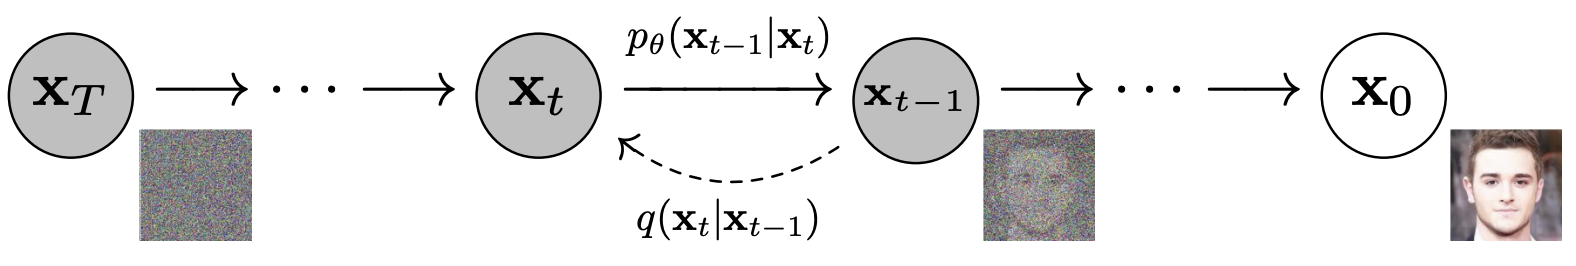
\includegraphics[width=1\linewidth]{figure/diffusion.png}
                    \caption{Diffusion. Image from Ho et al. (2020) - DDPM.}
                    \label{fig:diffusion}
                \end{figure}
				
				\note{Data distribution is slowly destroyed through an iterative forward diffusion process, then we learn a reverse diffusion process that restores structure in data. 
					  The forward diffusion process adds noise to the original image until it becomes pure noise, which converges to the normal distribution. 
					  Starting from a clean image $x_{0}$, we repeatedly add Gaussian noise at each time step. 
					  The amount of noise added at each time step can be controlled by the noise schedule, which determines how quickly the image becomes pure noise. 
					  As we continue adding noise, the image gradually loses its structure and eventually becomes indistinguishable from pure Gaussian noise. 
					  The reverse diffusion process involves training a neural network to learn to remove the noise step-by-step until we recover the clear image. 
					  Reverse process is done step-by-step because estimating small perturbations is more tractable than explicitly describing the full distribution. 
					  The neural network predicts the noise of the image, parameterized as a Gaussian distribution with learnable mean and variance.
					  The key insight is that by breaking down the generation process into many small denoising steps, we can learn complex distributions more effectively.}
            \end{frame}

            \begin{frame}{Probability Chain Rule}
                For any sequence of random variables $x_{0}, \cdots, x_{T}$, the joint distribution factorises as 
                $$p(x_0, \cdots, x_T) = p(x_{0}) p(x_{1} \mid x_{0}) p(x_{2} \mid x_{0}, x_{1}) \cdot \cdots \cdot p(x_{T} \mid x_{0:T-1})$$
                A process is Markov chain if the future depends only on the present, not the past:
                $$p(x_{t} \mid x_{0}, x_{1}, \cdots, x_{t - 1}) = p(x_{t} \mid x_{t - 1})$$
                Hence, the joint distribution reduces to 
                $$p(x_{0:T}) = p(x_{0}) \prod_{t=1}^T p(x_{t} \mid x_{t - 1})$$
                if it is Markovian.
				
				\note{The probability chain rule allows us to factorize joint distributions into products of conditional distributions. 
					  For a general sequence of random variables, each element can depend on all previous elements in the sequence. 
					  A Markov chain is a special case where each element depends only on the immediately previous element, not the entire history. 
					  This Markov property greatly simplifies the joint distribution, reducing it from a complex dependency structure to a simple product. 
					  In the context of diffusion models, the forward process is designed to be Markovian, meaning each noisy version depends only on the previous version. 
					  This Markov assumption makes the forward diffusion process tractable and allows us to sample noisy versions at any time step directly. 
					  The complete forward process can be written as a product of conditional probabilities, each depending only on the previous step. 
					  Similarly, the reverse process is also Markovian, with each denoising step depending only on the current noisy version. 
					  This Markov structure is crucial for making diffusion models computationally tractable. 
					  The simplification from general dependencies to Markov dependencies is what makes diffusion models practical for high-dimensional data.}
            \end{frame}

            \begin{frame}{Forward Process}
                \small
                By construction, the diffusion process follows the Markovian Gaussian distribution: 
                $$q(x_{t} \mid x_{t - 1}) = \mathcal{N}(\sqrt{\alpha_{t}} x_{t-1}, (1 - \alpha_{t})I) \; \badgeT$$ 
                where $\alpha_{t} = 1 - \beta_{t} \in [0, 1]$. \\
                Using the reparameterisation trick, $x_{t} = \sqrt{\alpha_{t}} x_{t - 1} + \sqrt{1 - \alpha_{t}} \cdot \epsilon_{t}$ where $\epsilon_{t} \sim \mathcal{N} (0, 1)$. \\
                Recursively,
                \begin{align*}
                    x_{t} & = \sqrt{\alpha_{1} \cdot \cdots \alpha_{t}} x_{0} + \sum_{s = 1}^{t} ((\sqrt{1 - \alpha_{s}} \prod_{j = s + 1}^{t} \sqrt{\alpha_{j}}) \cdot \epsilon_{s}) \\
                    & = \sqrt{\bar{\alpha}_{t}} x_{0} + \sqrt{1 - \bar{\alpha}_{t}} \cdot \epsilon 
                \end{align*}
                where $\bar{\alpha}_{t} = \prod_{s = 1}^{t} \alpha_{s}$ and $\epsilon \sim \mathcal{N} (0, 1)$. \\
                This implies 
                $$q(x_t \mid x_0) = \mathcal{N} (\sqrt{\bar{\alpha}_{t}}x_0, (1 - \bar{\alpha}_{t}) I) \; \badgeT \overset{t \to \infty}{\to} \mathcal{N} (0, I)$$
            
				\note{The forward diffusion process is designed as a Markov chain that gradually adds Gaussian noise. 
					  At each step, we add a small amount of noise scaled by $\alpha_t$, which controls the noise schedule. 
					  The conditional distribution $q(x_{t} \mid x_{t-1})$ is Gaussian with mean $\sqrt{\alpha_{t}} \times x_{t-1}$ and variance $1 - \alpha_{t}$. 
					  This formulation ensures that as $t$ goes to infinity, the distribution converges to a standard Gaussian, which becomes our prior. 
					  By using the reparameterization trick recursively, we can express the noisy version at any time step directly in terms of the original data. 
					  This direct connection allows us to sample noisy versions at any time step without going through all intermediate steps.}
			\end{frame}
    
            \begin{frame}{Reverse Process}
                True posterior can be defined as 
                $$q(x_{t - 1} \mid x_{t}, x_{0}) = \mathcal{N} (\tilde{\mu}_{t} (x_{t}, x_{0}), \tilde{\beta}_{t} I) \; \badgeT$$
                 where $\tilde{\mu}_{t} (x_{t}, x_{0}) = \frac{1}{\sqrt{\alpha_{t}}} (x_{t} - \frac{\beta_{t}}{\sqrt{1 - \bar{\alpha}_{t}}} \epsilon)$ with $\epsilon = \frac{x_{t} - \sqrt{\bar{\alpha}_{t}} x_{0}}{\sqrt{1 - \bar{\alpha}_{t}}}$ and $\tilde{\beta}_{t} = \frac{1 - \bar{\alpha}_{t - 1}}{1 - \bar{\alpha}_{t}} \beta_{t}$. \\
                 During the inference, $x_{0}$ is not accessible; hence, choose a Gaussian distribution
                 $$p_{\theta} (x_{t-1} \mid x_{t})= \mathcal{N} (\mu_{\theta} (x_{t}, t), \Sigma_{\theta}(x_{t}, t)) \; \badgeA$$
                 such that $\mu_{\theta}, \Sigma_{\theta}$ match the true posterior. \\
                 This is called a reverse kernel.
				 
				 \note{The reverse process in diffusion models aims to learn how to denoise and recover the original data. 
					   The true posterior $q(x_{t-1} \mid x_{t}, x_{0})$ is tractable if we condition on the original data $x_{0}$, but during generation we don't have access to it. 
					   By Bayes' rule, the true posterior can be written as a Gaussian distribution with a specific mean and variance. 
					   The mean $\tilde{\mu}_{t}$ depends on both the noisy image $x_{t}$ and the original clean image $x_{0}$. 
					   However, during inference when we want to generate new images, we don't have $x_0$, so we need to learn to approximate it. 
					   Instead, we learn a neural network that approximates this reverse process, parameterized by mean and variance functions $\mu_{\theta}$ and $\sigma_{\theta}$. 
					   The goal is to match the learned distribution $p_{\theta}(x_{t-1} \mid x_{t})$ to the true posterior $q(x_{t-1} \mid x_{t}, x_{0})$. 
					   This matching is what the training objective accomplishes, by minimizing the KL divergence between these distributions. 
					   The learned reverse kernel allows us to generate new images by starting from pure noise and iteratively applying the reverse process. 
					   The key challenge is that the network must learn to predict the denoising direction without knowing the original clean image, which is why we train it to match the true posterior that does have access to $x_{0}$.}
            \end{frame}

            \begin{frame}{Complete Process}
                \small
                Complete forward and reverse processes can be obtained using the probability chain rule. \\
                $$q(x_{1 : T} \mid x_{0}) = \prod_{t = 1}^{T} q(x_{t} \mid x_{t - 1})$$
                where $q(x_{t} \mid x_{t - 1}) = \mathcal{N} (\sqrt{\alpha_{t}} x_{t - 1}, \beta_{t} I)$, and
                $$p_{\theta} (x_{0:T}) = p(x_{T}) \prod_{t = 1}^{T}p_{\theta}(x_{t - 1} \mid x_{t})$$
                where $p(x_{T}) = \mathcal{N} (0, I)$. \\
				
				\note{The complete diffusion process consists of both forward and reverse processes defined through probability chain rules. 
					  The forward process takes clean data $x_{0}$ and gradually corrupts it with noise until we reach pure noise $x_{T}$. 
					  Each step in the forward process adds a small amount of Gaussian noise, with the noise schedule determining how much noise is added at each step. 
					  The complete forward process is the product of $T$ conditional distributions, each depending only on the previous step due to the Markov property. 
					  The reverse process learns to go from noise back to data, one denoising step at a time. 
					  The complete reverse process starts from pure Gaussian noise $p(x_T) = \mathcal{N}(0, I)$ and iteratively applies the learned reverse kernel. 
					  Each reverse step $p_{\theta}(x_{t-1} \mid x_{t})$ attempts to remove a small amount of noise, gradually recovering the clean image structure. 
					  The generation process starts from pure noise and iteratively applies the learned reverse kernel to produce clean data. 
					  The key difference is that the forward process is deterministic given the noise schedule, while the reverse process must be learned from data. 
					  This formulation allows us to train the model using the forward process to create training pairs, and then learn the reverse process to generate new samples.}
            \end{frame}

            \begin{frame}{Objective}
                \begin{align*}
                    \log{p_{\theta} (x_{0})} & = \log{\int p_{\theta} (x_{0:T}) dx_{1:T}} \\
                    & \geq \mathbb{E}_{q(x_{1:T} \mid x_{0})} [\log{\frac{p_{\theta} (x_{0:T})}{q(x_{1:T} \mid x_{0})}}] \\
                    & = \underbrace{\mathbb{E}_{q(x_{1} \mid x_{0})} [\log{p_{\theta} (x_{0} \mid x_{1})}]}_{\text{Reconstruction term \; \badgeA}} - \underbrace{D_{\mathrm{KL}} (q(x_{T} \mid x_{0}) \Vert p(x_{T}))}_{\text{Prior matching term}} \\ 
                    & \quad - \underbrace{\sum_{t = 2}^{T} \mathbb{E}_{q(x_{1:T} \mid x_{0})} [D_{\mathrm{KL}} (q(x_{t - 1} \mid x_{t}, x_{0}) \Vert p_{\theta}(x_{t - 1} \mid x_{t}))]}_{\text{Denoising matching term} \; \badgeT}
                \end{align*}    
				
				\note{The diffusion training objective is derived by applying variational inference to bound the log-likelihood. 
					  We want to maximize the log-likelihood of the data, but this is intractable, so we derive a lower bound using Jensen's inequality. 
					  The bound decomposes into three terms: a reconstruction term, a prior matching term, and a denoising matching term. 
					  The reconstruction term measures how well the model can reconstruct the original data from the first noisy version. 
					  The prior matching term ensures that after T steps of forward diffusion, the distribution matches our prior, which is standard Gaussian noise. 
					  The denoising matching term is the most important, requiring the model to match the true posterior at each noise level. 
					  This term is the sum of KL divergences between the true posterior $q(x_{t-1} \mid x_{t}, x_{0})$ and the learned reverse process$p_{\theta}(x_{t-1} | x_{t})$. 
					  The true posterior is called the teacher distribution because it has access to the original clean image $x_{0}$ during training. 
					  The whole point is to train the neural network to match the true posterior, so that during inference it can denoise effectively without knowing $x_{0}$. 
					  This matching ensures that the learned reverse process can effectively denoise at every step of the process.}
            \end{frame}

            \begin{frame}{Simplified Objective}
                KL Divergence between two Gaussian distributions is 
                $$D_{\mathrm{KL}} (\mathcal{N} (\mu_{x}, \Sigma_{x}) \Vert \mathcal{N} (\mu_{y}, \Sigma_{y})) = \frac{1}{2}[\log{\frac{\lvert \Sigma_{y} \rvert}{\lvert \Sigma_{x} \rvert}} - d + tr(\Sigma_{y}^{-1} \Sigma_{x}) + (\mu_{y} - \mu_{x})^{T} \Sigma_{y}^{-1} (\mu_{y} - \mu_{x})]$$
                KL term reduces to expectations of squared errors between true $\tilde{\mu}$ and predicted means $\mu_{\theta}$. \\
                Simplified loss is given by 
                $$\mathcal{L} (\theta) = \mathbb{E} [\frac{\beta_{t}^{2}}{2 \sigma_{t}^{2} \alpha_{t} (1 - \bar{\alpha_{t}})} \Vert \epsilon - \epsilon_{\theta} (x_{t}, t)\Vert^{2}] \; \badgeT$$
                where $x_{t} = \sqrt{\bar{\alpha}_{t}} x_{0} + \sqrt{1 - \bar{\alpha}_{t}} \epsilon$ with $\epsilon \sim \mathcal{N} (0, I)$.
            
				\note{The diffusion objective can be simplified by computing the KL divergence between Gaussian distributions. 
					  The KL divergence between two Gaussians has a closed-form expression involving the means and covariances. 
					  For the diffusion model, we typically set the covariance to be fixed, so the KL term reduces to squared errors between the true and predicted means. 
					  The true mean $\tilde{\mu}_{t}$ can be expressed in terms of the noise $\epsilon$ that was added to create $x_{t}$ from $x_{0}$. 
					  Instead of predicting the mean directly, we can predict the noise $\epsilon_{\theta}$, which is equivalent but often more stable. 
					  The final simplified loss is a weighted mean squared error between the true noise and predicted noise at each time step. 
					  The weight depends on the noise schedule parameters and ensures that all time steps contribute appropriately to the loss. 
					  This formulation is much simpler to implement and optimize than the original KL divergence formulation. 
					  The network learns to predict the noise that was added at each step, which is easier than predicting the mean directly. 
					  This simplified objective contributed significantly to the success of diffusion models, making them practical to train on large datasets.}
			\end{frame}

        \subsection{Score-Based Models}
            \begin{frame}{Intuition}
                \begin{figure}
                    \centering
                    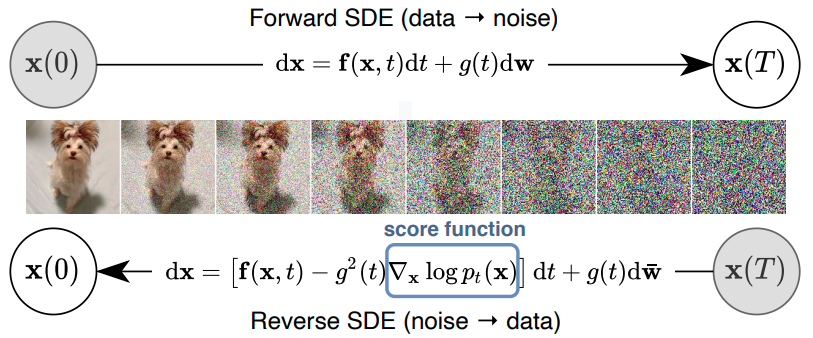
\includegraphics[width=0.8\linewidth]{figure/score_matching.png}
                    \caption{Score matching. Image from Song et al. (2020) – Score-Based Generative Model through SDE.}
                    \label{fig:score_matching}
                \end{figure}
				
				\note{Score-based models learn the score function, which is the gradient of the log-probability with respect to the data. 
					  The score function tells us the direction of steepest increase in probability, pointing toward modes of the distribution. 
					  This approach is appealing because we can work with unnormalized distributions - we don't need the partition function. 
					  The connection to denoising is key: estimating the score is equivalent to learning to denoise, which is more tractable than learning the full distribution. 
					  Score-based models generalize diffusion models by working in continuous time rather than discrete steps. 
					  They use stochastic differential equations or SDEs to describe the forward noising process and the reverse generation process. 
					  The score function naturally connects to energy-based models, as the score equals the negative gradient of the energy. 
					  This connection allows score-based models to work with unnormalized distributions, avoiding the partition function problem. 
					  The key insight is that learning to estimate scores is more tractable than learning full probability distributions. 
					  Score-based models have achieved impressive results in image generation and have been shown to be equivalent to diffusion models under certain conditions.}
            \end{frame}

            \begin{frame}{Score Function}
                For a probability density $p(x)$, the score function is 
                $$s(x) = \nabla_{x} \log{p(x)}$$
                which tells which direction in data space increases probability the fastest. \\
                At the mode of the distribution, the score is zero. \\
                For the case of EBM, $s(x) = - \nabla_{x} E(x)$, which removes the necessity of computing $Z(\theta)$. 
            
				\note{The score function is defined as the gradient of the log-density with respect to the data. 
					  At modes of the distribution, where probability is highest, the score is zero. 
					  For energy-based models, the score equals the negative gradient of the energy, providing a direct connection. 
					  This connection is powerful because we can learn scores without computing the intractable partition function. 
					  The score function tells us which direction in data space increases probability the fastest. 
					  This is particularly useful for sampling, as we can use the score to guide samples toward high-probability regions. 
					  The score function is a vector field that points toward modes of the distribution. 
					  Learning the score function is often easier than learning the full probability distribution, especially for high-dimensional data. 
					  The score function appears naturally in many probabilistic models, including diffusion models and energy-based models. 
					  Understanding the score function is crucial for understanding how score-based models work and how they relate to other generative model families.}
			\end{frame}

            \begin{frame}{Tweedie's Formula}
                Suppose the data is corrupted by Gaussian noise, i.e. $x = x_{0} + \sigma \epsilon$ where $\epsilon \sim \mathcal{N} (0, I)$. \\
                Then the Tweedie's formula says
                $$\mathbb{E} [x_{0} \mid x] = x + \sigma^2 \nabla_x \log p_\sigma(x)$$ 
                where $p_{\sigma} (x)$ is the marginal distribution of noisy observations. \\
                Posterior mean is given by the noisy point $x$ and a correction from the score. \\
                Since the posterior mean is the best possible estimate of $x_{0}$ given noisy observation $x$, denoising is equivalent to estimating a score function. 
            
				\note{Tweedie's formula provides a beautiful connection between denoising and score estimation. 
					  When data is corrupted by Gaussian noise, the optimal denoising estimate involves the score function. 
					  The posterior mean can be expressed as the noisy point plus a correction term involving the score. 
					  This means that learning to denoise is equivalent to learning the score function, which is why score-based models are so effective. 
					  Tweedie's formula shows that the optimal denoising estimate is the noisy point plus sigma squared times the score. 
					  This formula connects the score function to denoising, showing that score estimation is fundamentally a denoising problem. 
					  The posterior mean is the best possible estimate of the clean data given the noisy observation. 
					  Since the posterior mean involves the score function, denoising is equivalent to estimating a score function. 
					  This connection is why score-based models can be trained using denoising objectives. 
					  Understanding Tweedie's formula helps us see why score-based models work so well and how they relate to diffusion models.}
			\end{frame}

            \begin{frame}{Fisher Divergence}
                Just like KL divergence, the Fisher divergence
                $$D_{\textrm{F}} (p \Vert p_{\theta}) = \mathbb{E}_{x \sim p(x)} [ \Vert \nabla_{x} \log{p(x)} - \nabla_{x} \log{p_\theta(x)} \Vert^{2}]$$
                measures the closeness of two score functions. 
				
				\note{Fisher divergence measures the distance between two distributions through their score functions. 
					  Like KL divergence, it quantifies how close two distributions are, but focuses on the gradients rather than the densities themselves. 
					  This is particularly useful when we can't compute densities but can estimate their gradients. 
					  The Fisher divergence naturally appears when we try to match score functions rather than densities directly. 
					  The Fisher divergence is defined as the expected squared difference between the score functions of the true and model distributions. 
					  This metric is particularly useful for score-based models, where we work with score functions rather than densities. 
					  The Fisher divergence has nice properties, including being symmetric and having a clear geometric interpretation. 
					  Unlike KL divergence, Fisher divergence doesn't require computing the full density, making it more tractable for some applications. 
					  Understanding Fisher divergence helps us understand how score-based models are trained and evaluated. 
					  This metric connects score-based models to other probabilistic models and provides a principled way to measure distribution differences.}
            \end{frame}

            \begin{frame}{Objective}
                Directly minimising $D_{\textrm{F}}$ requires the true score $s(x) \; \badgeI$, which is unknown. \\  
                Hyvärinen (2005) showed an equivalent, tractable objective:
                $$J(\theta) = \mathbb{E}_{x \sim p(x)} [\frac{1}{2} \Vert s_\theta(x) \Vert^{2} + \mathrm{tr}{(\nabla_x s_\theta(x))]} \; \badgeT$$
                This only uses data samples $x \sim p(x)$ and the model score $s_\theta(x)$.
				
				\note{Directly minimizing Fisher divergence requires the true score function, which we don't have. 
					  However, Hyvärinen showed that we can derive an equivalent objective that only requires samples from the data distribution. 
					  This objective involves the squared norm of the model score plus its divergence, which can both be computed. 
					  This tractable objective allows us to train score-based models using only data samples, without needing the true distribution. 
					  The key insight is that we can compute the divergence of the score function using only the model and data samples. 
					  This objective is much more tractable than trying to compute the Fisher divergence directly. 
					  The divergence term acts as a regularizer, encouraging the score function to be well-behaved. 
					  This formulation makes score-based models practical to train on large datasets. 
					  Understanding this objective is crucial for understanding how score-based models are trained. 
					  he tractability of this objective is one of the key advantages of score-based models over other approaches.}
            \end{frame}

            \begin{frame}{Forward Process}
                Score-based models describe data noising by an Itô SDE:
                $$dx = f(x,t)\,dt + g(t)\,dW_t $$
                where $f(x, t)$ is the drift term (deterministic), $g(t)$ is the diffusion strength, and $W_{t}$ is the Wiener process or Brownian motion (stochastic). \\
                
                \begin{itemize}
                    \item Variance-preserving (VP) SDE: \\ 
                    $dx = -\frac{1}{2} \beta (t)x \; dt + \sqrt{\beta(t)} \; dW_{t} \Longrightarrow x_{t} = \sqrt{\alpha_{t}} x_{0} + \sqrt{1 - \alpha_{t}} \epsilon$ with $\alpha_{t} = \exp{(- \int_{0}^{t} \beta(s) ds)}$
                    \item Variance-exploding (VE) SDE: \\ 
                    $dx = g(t) \; dW_t \Longrightarrow x_{t} = x_{0} + \sigma (t) \epsilon$ with $\sigma (t) = \int_{0}^{t} g^{2} (s) ds$
                \end{itemize}
				
				\note{Score-based models describe the forward noising process using stochastic differential equations or SDEs. 
					  SDEs generalize diffusion models by allowing more flexible noise schedules and drift terms. 
					  The forward SDE describes how data is gradually corrupted with noise over continuous time. 
					  Variance-preserving SDEs maintain variance while adding noise, similar to standard diffusion models. 
					  Variance-exploding SDEs allow variance to grow, which can be more effective for certain types of data. 
					  The drift term $f(x, t)$ describes deterministic evolution, while the diffusion term $g(t)$ controls noise strength. 
					  The Wiener process $W_{t}$ represents Brownian motion, providing the stochastic component. 
					  This continuous-time formulation is more flexible than discrete diffusion models. 
					  The SDE formulation allows us to work with different noise schedules and diffusion strengths. 
					  Understanding the forward SDE is crucial for understanding how score-based models work and how they relate to diffusion models.}
            \end{frame}

            \begin{frame}{Reverse Process}
                Anderson (1982) proved that if $\{ x_{t} \}_{t \in [0, T]}$ follows the forward SDE with marginal distribution $p(x)$, the time reversed process is also an SDE:
                $$dx = [f(x,t) - g^{2}(t) \; s(x,t)] dt + g(t) \; d \bar{W_{t}}$$
                where $\bar{W_{t}}$ is a Brownian motion in reverse time.
				
				\note{Anderson's theorem provides the mathematical foundation for reversing SDEs. 
					  The reverse process is also an SDE, but with a modified drift term that includes the score function. 
					  This score term acts as a correction that guides the reverse process toward high-probability regions. 
					  The reverse SDE can be solved numerically to generate samples, though this requires careful discretization. 
					  The drift term in the reverse SDE is the original drift minus g squared times the score function. 
					  This correction term ensures that the reverse process generates samples from the correct distribution. 
					  The Brownian motion in reverse time is different from forward time, but has the same statistical properties. 
					  The reverse SDE shows how to generate samples by starting from noise and following the reverse process. 
					  This formulation unifies many generative modeling approaches, including diffusion models and energy-based models. 
					  Understanding the reverse SDE is crucial for understanding how score-based models generate samples.}
            \end{frame}

            \begin{frame}{Langevin Dynamics}
                \footnotesize
                Langevin dynamics provides how particles move in a fluid, where they feel both deterministic forces and random collisions. \\
                The general Langevin equation for a particle with mass $m$ is given as
                $$m \frac{d^{2}x}{dt^{2}} = -\gamma \frac{dx}{dt} - \nabla U(x) + \sqrt{2 \gamma k_{B} T} \xi (t)$$
                where $-\gamma \dot{x}$ is the friction or damping term, $-\nabla U(x)$ is the deterministic force from potential energy $U(x)$, and $\sqrt{2 \gamma k_{B} T} \xi (t)$ is the thermal noise. \\
                Overdamped Langevin dynamics in terms of probability density $p(x) \propto e^{-U(x)}$ can be written as 
                $$dx = \nabla_{x} \log{p(x)} \; dt + \sqrt{2} \; dW_{t}$$
                Discretised case for sampling is given by Euler-Maruyama equation
                $$x_{k + 1} = x_{k} + \eta \nabla_{x} \log{p(x_{k})} + \sqrt{2 \eta} z_{k}$$ 
                with $z_{k} \sim \mathcal{N} (0, I)$ where $\eta$ is the step size.
				
				\note{Langevin dynamics describes how particles move in a fluid under both deterministic forces and random thermal motion. 
					  The equation balances friction, deterministic forces from potential energy, and stochastic noise. 
					  In the overdamped limit, this simplifies to a first-order equation involving the gradient of the log-probability. 
					  For sampling, we discretize this equation, creating a Markov chain that samples from the distribution. 
					  The overdamped Langevin dynamics can be written in terms of the score function, which is the gradient of the log-probability. 
					  This connects Langevin dynamics to score-based models, as both use the score function for sampling. 
					  The discretization uses the Euler-Maruyama scheme, which approximates the continuous SDE with discrete steps. 
					  Langevin dynamics provides a way to sample from distributions using only the score function. 
					  This is particularly useful for energy-based models, where we can compute the score from the energy function. 
					  Understanding Langevin dynamics helps us understand how score-based models generate samples and how they relate to other sampling methods.}
            \end{frame}

            \begin{frame}{Predictor-Corrector Samplers}
                Direct discretisation can produce unstable samples. \\
                The predictor-corrector method improves stability by alternating 

                \begin{itemize}
                    \item Predictor step: Move sample along reverse SDE (Global trajectory)
                    \item Corrector step: Refine sample with Langevin dynamics (Local adjustment)
                \end{itemize}
				
				\note{Predictor-corrector methods improve sampling stability by combining global and local updates. 
					  The predictor step follows the reverse SDE, giving a global trajectory through the space. 
					  The corrector step uses Langevin dynamics to refine the sample locally, improving accuracy. 
					  This alternation between global and local updates produces more stable and higher-quality samples than either method alone. 
					  Direct discretization of the reverse SDE can produce unstable samples, especially when the score function is inaccurate. 
					  The predictor step moves the sample along the reverse SDE trajectory, providing a global update. 
					  The corrector step uses Langevin dynamics to refine the sample locally, correcting for discretization errors. 
					  This combination allows for more accurate sampling while maintaining stability. 
					  Predictor-corrector methods are particularly important for score-based models, where accurate sampling is crucial. 
					  Understanding these methods helps us understand how to generate high-quality samples from score-based models.}
            \end{frame}

        \subsection{Generative Adversarial Network (GAN)}
            \begin{frame}{Intuition}
                \begin{figure}
                     \centering
                     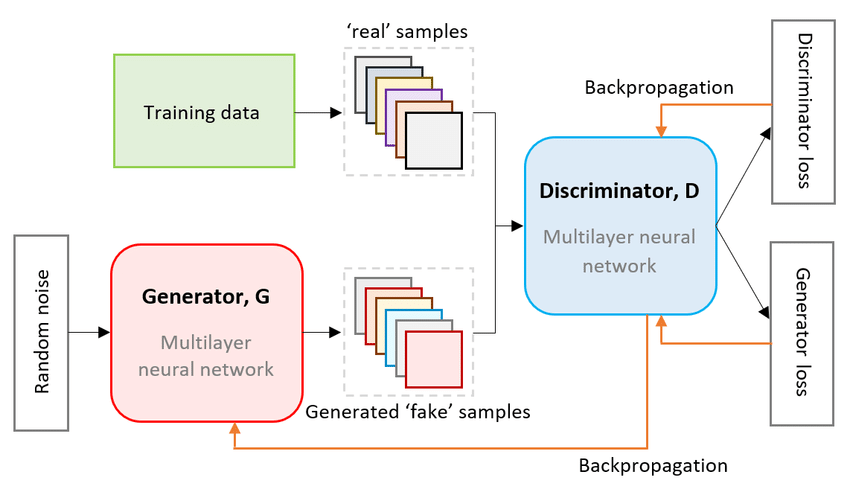
\includegraphics[width=0.7\linewidth]{figure/gan.png}
                     \caption{GAN. Image from Little et al. (2021) – Generative Adversarial Networks for Synthetic Data Generation.}
                     \label{fig:gan}
                 \end{figure} 
				 
				 \note{GANs use an adversarial game between two networks: a generator and a discriminator. 
					   The generator tries to create fake samples that fool the discriminator, while the discriminator tries to distinguish real from fake. 
					   This adversarial training creates a competitive dynamic that drives both networks to improve. 
					   Unlike other generative models, GANs don't explicitly model likelihoods, making them implicit generative models. 
					   The generator maps noise to fake samples, trying to create a distribution that matches the data. 
					   The discriminator outputs a probability that an input is real, trying to correctly classify samples. 
					   This adversarial process leads to both networks improving their capabilities over time. 
					   GANs have achieved remarkable success in generating high-quality images, videos, and other data types. 
					   The key advantage is that they can generate sharp, high-fidelity samples in a single forward pass. 
					   However, GANs are notoriously difficult to train, often suffering from mode collapse and training instability.}
            \end{frame}

            \begin{frame}{Minimax Game}
                \begin{itemize}
                    \item Generator $G(z)$: Map noise $z \sim p(z)$ to fake samples, inducing distribution $p_{g}(x) \; \badgeI$. 
                    \item Discriminator $D(x)$: Output probability that $x$ is real
                    \item Value function: $\underset{G}{\min} \underset{D}{\max} V(D, G) = \mathbb{E}_{x \sim p(x)} [\log D(x)] + \mathbb{E}_{z \sim p(z)} [\log(1 - D(G(z)))] \; \badgeT$
                \end{itemize}            
				
				\note{The GAN training is formulated as a minimax game where the generator and discriminator have opposing objectives. 
					  The generator maps noise to fake samples, trying to create a distribution that matches the data. 
					  The discriminator outputs a probability that an input is real, trying to correctly classify samples. 
					  The value function captures this adversarial relationship, with the generator minimizing and discriminator maximizing. 
					  The minimax formulation means the generator tries to minimize the value function while the discriminator tries to maximize it. 
					  This creates a competitive dynamic where both networks improve their capabilities. 
					  The Nash equilibrium of this game occurs when the generator perfectly matches the data distribution and the discriminator becomes a random guesser. 
					  The value function is based on binary cross-entropy, treating real vs fake as a binary classification problem. 
					  This formulation makes GAN training a zero-sum game, where one network's gain is the other's loss. 
					  Understanding the minimax game is crucial for understanding how GANs work and why they can be difficult to train.}
            \end{frame}

            \begin{frame}{Objective}
                Binary cross entropy is given by $BCE(y, D(x)) = -y \log{D(x)} - (1 - y) \log{(1 - D(x))}$. \\
                If the sample is real $(y = 1)$, the loss is $- \log{D(x)}$ and if it is fake $(y = 0)$, the loss is $- \log{(1 - D(x))}$. \\
                Discriminator's objective is
                $$\mathcal{L} (D) = - \mathbb{E}_{x \sim p(x)} [\log{D(x)}] - \mathbb{E}_{z \sim p(z)} [\log{(1 - D(G(z)))}]$$
                Generator's objective is 
                $$\mathcal{L} (G) = \mathbb{E}_{z \sim p(z)} [\log{(1 - D(G(z)))}]$$
                Note that when $D(G(z)) \to 0$, the gradient vanishes; flip the label to 1 for fake samples, i.e., 
                $$\mathcal{L} (G) = - \mathbb{E}_{z \sim p(z)} [\log{D(G(z))}]$$
				
				\note{The GAN objectives are derived from binary cross-entropy, treating real vs fake as a binary classification problem. 
					  The discriminator's loss is the standard binary cross-entropy for distinguishing real from generated samples. 
					  The generator's loss initially uses the same formulation, but this can lead to vanishing gradients when the discriminator is too good. 
					  To fix this, we flip the labels for fake samples, so the generator maximizes the discriminator's probability that fakes are real. 
					  When the discriminator is too confident, the gradient for the generator becomes very small, making training difficult. 
					  By flipping the labels, we ensure the generator always has a strong gradient signal, even when the discriminator is very good. 
					  This modification makes GAN training more stable and allows the generator to learn effectively. 
					  The discriminator's objective is to maximize the log probability of real samples and minimize the log probability of fake samples. 
					  The generator's objective is to maximize the log probability that its generated samples are classified as real. 
					  This formulation creates a competitive dynamic that drives both networks to improve their capabilities.}
            \end{frame}

            \begin{frame}{Optimal Solution}
                \footnotesize
                Setting $p_{g}(x)$ fixed, then 
                $$f(x) = p(x) \log{D(x)} + p_{g}(x)\log{(1 - D(x))}$$ \\
                $$\frac{\partial f}{\partial D} = \frac{p(x)}{D(x)} - \frac{p_{g}(x)}{1 - D(x)} = 0 \iff D^{*}(x) = \frac{p(x)}{p(x) + p_{g}(x)}$$
                where $D^{*}$ is the optimal discriminator. \\
                Introduce a mixture distribution $M(x) = \frac{1}{2} (p(x) + p_{g}(x))$, then the value function reduces to 

                \begin{align*}
                    V(D^{*},G) & = \mathbb{E}_{p} [\log{\frac{p(x)}{M(x)}}] + \mathbb{E}_{p_g} [\log{\frac{p_g(x)}{M(x)}}] - 2 \log{2} \\
                    & = D_{\mathrm{KL}} (p(x) \Vert M(x)) + D_{\textrm{KL}} (p_{g}(x) \Vert M(x)) - 2 \log{2} \\
                    & = - \log{4} + 2 D_{\textrm{JS}} (p(x) \Vert p_{g}(x))
                \end{align*}
                where $D_{\mathrm{JS}}(p \Vert p_g) = \frac{1}{2} D_{\mathrm{KL}} (p \Vert M) + \frac{1}{2} D_{KL} (p_g \Vert M)$ is the Jensen-Shannon divergence. \\
                At the global optimum, $p_{g} (x) = p(x)$, $D_{\mathrm{JS}} = 0$, and $V(D^{*},G) = - \log{4}$.
            
				\note{The optimal discriminator has a closed-form solution in terms of the true and generated distributions. 
					  When we plug this optimal discriminator into the value function, it reduces to a Jensen-Shannon divergence. 
					  This shows that the GAN game is fundamentally about minimizing JS divergence between the true and generated distributions. 
					  At the global optimum, the generator perfectly matches the data distribution, and the discriminator becomes a random guesser. 
					  The optimal discriminator outputs the ratio of the true distribution to the sum of true and generated distributions. 
					  This optimal solution shows that perfect training would lead to the generator matching the data distribution exactly. 
					  The value function at the optimum is negative log 4, which occurs when the JS divergence is zero. 
					  This theoretical result provides important insights into what GANs are trying to achieve. 
					  However, in practice, achieving this optimum is very difficult due to training instabilities. 
					  Understanding the optimal solution helps us understand the theoretical foundations of GANs and why they can be difficult to train.}
			\end{frame}

    \section{Summary}
        \begin{frame}{Architecture}
            \begin{figure}
                \centering
                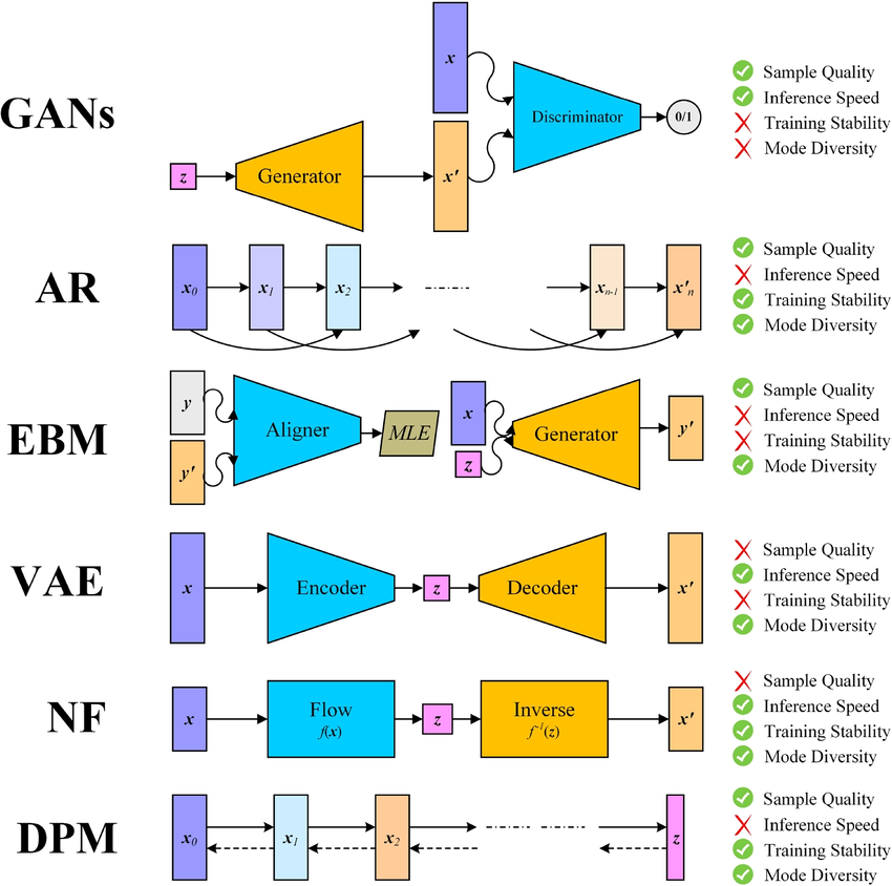
\includegraphics[width=0.4\linewidth]{figure/architecture.png}
                \caption{Architecture of different generative models. Image from Ahmad et al. (2024) – Understanding GANs.}
                \label{fig:architecture}
            \end{figure}
			
			\note{This slide shows the architectural differences between various generative model families. 
				  Explicit models like VAEs and normalizing flows have clear encoder-decoder or flow structures. 
				  Implicit models like GANs have generator-discriminator pairs. 
				  Score-based models learn score networks, while diffusion models have denoising networks. 
				  Each architecture reflects how the model handles the fundamental challenge of modeling complex distributions. 
				  The encoder-decoder structure in VAEs allows for efficient encoding and decoding of data. 
				  The flow structure in normalizing flows ensures invertibility and tractable likelihood computation. 
				  The generator-discriminator structure in GANs enables adversarial training without explicit likelihoods. 
				  The denoising network in diffusion models learns to reverse the forward diffusion process. 
				  Understanding these architectural differences helps us understand the strengths and limitations of each approach.}
        \end{frame}

        \begin{frame}{Model Landscape}
            \tiny
            \renewcommand{\arraystretch}{1.3}
            \begin{tabularx}{\linewidth}{@{} l l X @{}}
                \toprule
                \textbf{Family} & \textbf{Model} & \textbf{Key Idea} \\
                \midrule
                Explicit (factorized) & ARM &
                \begin{itemize}
                  \item Chain-rule factorisation of joint distribution
                \end{itemize} \\
                Explicit (latent) & VAE &
                \begin{itemize}
                  \item Latent variables + variational inference (ELBO)
                  \item Balances reconstruction and regularisation
                \end{itemize} \\
                Explicit (invertible) & Normalising Flow &
                \begin{itemize}
                  \item Sequence of invertible maps with tractable Jacobians
                  \item Discrete-step explicit density model
                \end{itemize} \\
                Continuous flows & Flow Matching (ODE) &
                \begin{itemize}
                  \item Continuous analogue of flows via velocity fields
                  \item Generalises diffusion without discrete Markov chain
                \end{itemize} \\
                Score/Energy & EBM &
                \begin{itemize}
                  \item Defines unnormalised density via energy
                  \item Direct link to score: $s(x) = -\nabla E(x)$
                \end{itemize} \\
                Score/Energy & Diffusion (DDPM) &
                \begin{itemize}
                  \item Discrete Markov noise process
                \end{itemize} \\
                Score/Energy & Score-Based (SDE) &
                \begin{itemize}
                  \item Learns time-dependent scores $s(x,t)$
                  \item Reverse-time SDE unifies with EBMs/diffusion
                \end{itemize} \\
                Implicit (adversarial) & GAN &
                \begin{itemize}
                  \item No explicit likelihood
                  \item Adversarial game to match data distribution
                \end{itemize} \\
                \bottomrule
            \end{tabularx}
			
			\note{This table organizes generative models into families based on their mathematical foundations. 
				  Explicit models with factorizations include autoregressive models that use chain rule factorizations. 
				  Latent variable models like VAEs use variational inference with ELBO objectives. 
				  Implicit models like GANs use adversarial training without explicit likelihoods. 
				  Understanding these families helps us see the fundamental trade-offs in generative modeling. 
				  Each family has its own approach to handling the normalization constraint and computing likelihoods. 
				  Explicit models allow us to compute likelihoods but often require approximations. 
				  Implicit models can generate high-quality samples but don't provide likelihood estimates. 
				  The continuous flow models provide a bridge between discrete and continuous approaches. 
				  This landscape helps us understand when to use each type of model for different applications.}
        \end{frame}

        \begin{frame}{Comparison of Generative Models (1/2)}
            \tiny
            \renewcommand{\arraystretch}{1.3}
            \begin{tabularx}{\linewidth}{@{} l X X @{}}
                \toprule
                \textbf{Model} & \textbf{Pros} & \textbf{Cons} \\ 
                \midrule
                ARM &
                \begin{itemize}\item Exact likelihood \item Stable MLE training \item Strong for sequential data \end{itemize} &
                \begin{itemize}\item Slow sequential sampling \item Limited parallelism \item Exposure bias \end{itemize} \\
                VAE &
                \begin{itemize}\item Learns latent representations \item Tractable ELBO \item Smooth interpolation \end{itemize} &
                \begin{itemize}\item Variational gap \item Blurry reconstructions \item Posterior mismatch \end{itemize} \\
                Normalising Flow &
                \begin{itemize}\item Exact log-likelihood \item Fast inference \item Principled density modeling \end{itemize} &
                \begin{itemize}\item Invertibility/Jacobian constraints \item Limited expressivity on complex data \end{itemize} \\
                Flow Matching (ODE) &
                \begin{itemize}\item Direct continuous path \item Simple MSE training \item Fewer steps than diffusion \end{itemize} &
                \begin{itemize}\item Requires tractable conditional velocities \item Still new; fewer benchmarks \end{itemize} \\
                \bottomrule
            \end{tabularx}
        \end{frame}

        \begin{frame}{Comparison of Generative Models (2/2)}
            \tiny
            \renewcommand{\arraystretch}{1.3}
            \begin{tabularx}{\linewidth}{@{} l X X @{}}
                \toprule
                \textbf{Model} & \textbf{Pros} & \textbf{Cons} \\ 
                \midrule
                EBM &
                \begin{itemize}\item Very flexible (no invertibility/latent vars) \item Natural physics analogy \item Connects to scores \end{itemize} &
                \begin{itemize}\item Partition function intractable \item Requires expensive MCMC \item Training unstable at scale \end{itemize} \\
                Diffusion (DDPM) &
                \begin{itemize}\item State-of-the-art fidelity \item Stable training \item Likelihood surrogate (ELBO) \end{itemize} &
                \begin{itemize}\item Very slow sampling (many steps) \item Careful noise schedule required \end{itemize} \\
                Score-Based (SDE) &
                \begin{itemize}\item Unifies diffusion/EBM/Langevin \item Flexible SDE choices \item High quality with PC samplers \end{itemize} &
                \begin{itemize}\item Training across many noise levels \item Sampling slower than ARMs/GANs \end{itemize} \\
                GAN &
                \begin{itemize}\item Sharp, high-fidelity one-shot samples \item Very fast generation \end{itemize} &
                \begin{itemize}\item Training instability (mode collapse) \item No explicit likelihood \item Sensitive to hyperparameters \end{itemize} \\
                \bottomrule
            \end{tabularx}
        \end{frame}
\end{document}